\documentclass[10pt,onecolumn,A4]{article}


\usepackage{times}
\usepackage{epsfig}
\usepackage{graphicx}
\usepackage{amsmath}
\usepackage{amssymb}

% usepackages by Petr
\usepackage{epstopdf}
\usepackage{enumerate}
\usepackage{subfigure}
\usepackage{caption}
\usepackage{tabularx}
\usepackage[table]{xcolor}
\usepackage{hyphenat}
\setlength\textwidth{175mm}
\setlength\textheight{280mm}
\setlength\oddsidemargin{0mm}
\setlength\evensidemargin{0mm}
\setlength\topmargin{-25mm}
\setlength\headsep{0mm}
\setlength\headheight{0mm}
\setlength\leftmargin{0mm}

\definecolor{myGrey}{HTML}{33FF00}
\definecolor{myRed}{HTML}{FF3030}
\definecolor{myGreen}{HTML}{00FF00}
\definecolor{myGrey}{HTML}{AAAAAA}
\definecolor{myWhite}{HTML}{FFFFFF}
\definecolor{myCopper1}{HTML}{FFC77F}
\definecolor{myCopper2}{HTML}{FFAB6D}
\definecolor{myCopper3}{HTML}{E9915D}
\definecolor{myCopper4}{HTML}{BB754B}
\definecolor{myCopper5}{HTML}{935C3A}


\title{Supplementary material for submission \# 954\\
Fisher vector places: learning compact descriptors for place recognition
 }
\begin{document}
	\maketitle

\begin{figure}
	\center
	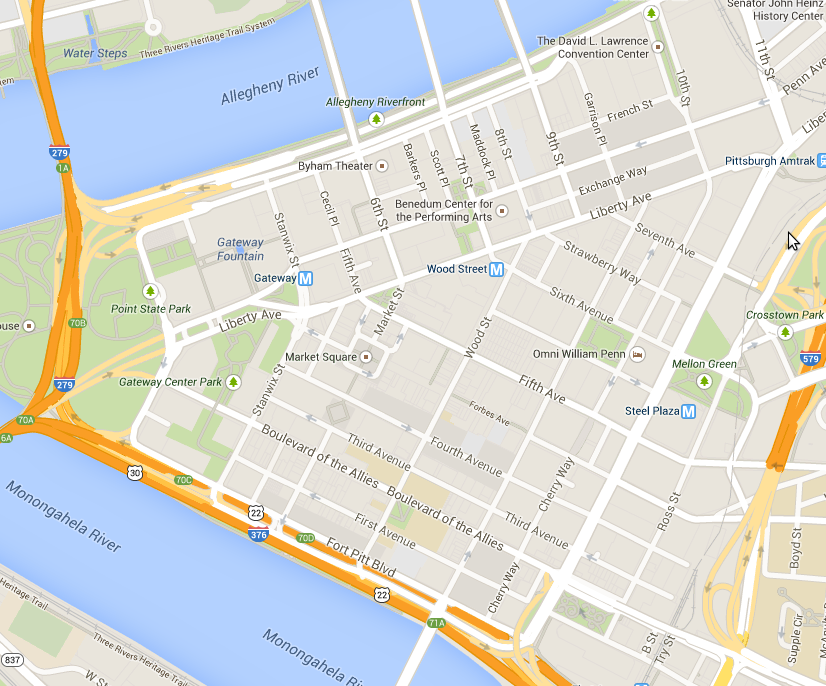
\includegraphics[trim = 55mm 40mm 55mm 25mm, clip=true,width=0.5\linewidth]{mapGoogle.png}
	\caption{ \textbf{A map corresponding to the area covered by image database.}
		The Pittsburgh 25k dataset covers roughly an area of $1.3 \times 1.2 \; {\rm km}^2$.
	}
\end{figure}

\begin{figure}
	\begin{minipage}{0.45\linewidth}
		\center
		FV128 (baseline, no learning) \\
		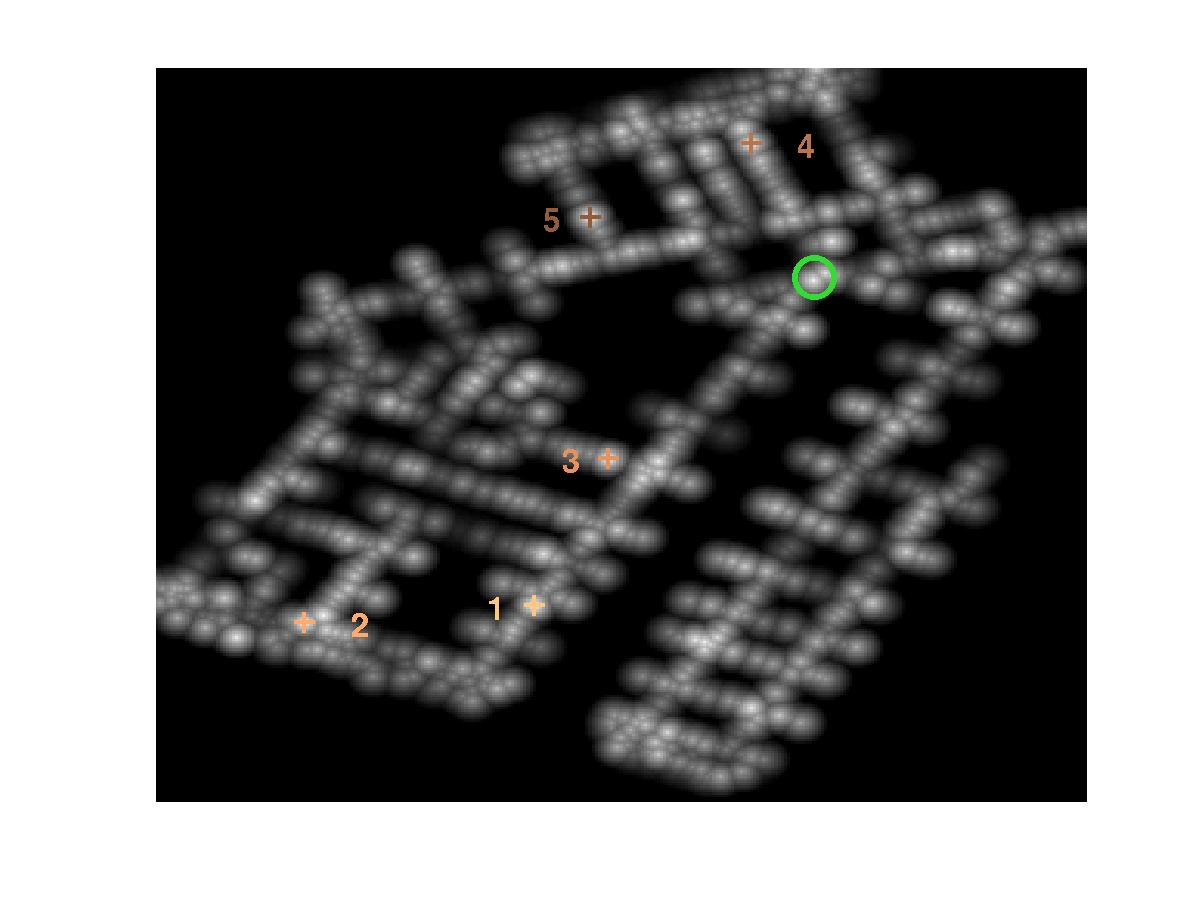
\includegraphics[trim = 55mm 40mm 55mm 25mm, clip=true,width=\linewidth]{sup1383/heatRaw.jpg}
	\end{minipage} 
	\begin{minipage}{0.45\linewidth}
		\center
		FV128 e-SVM (proposed learnt compact descriptor) \\
		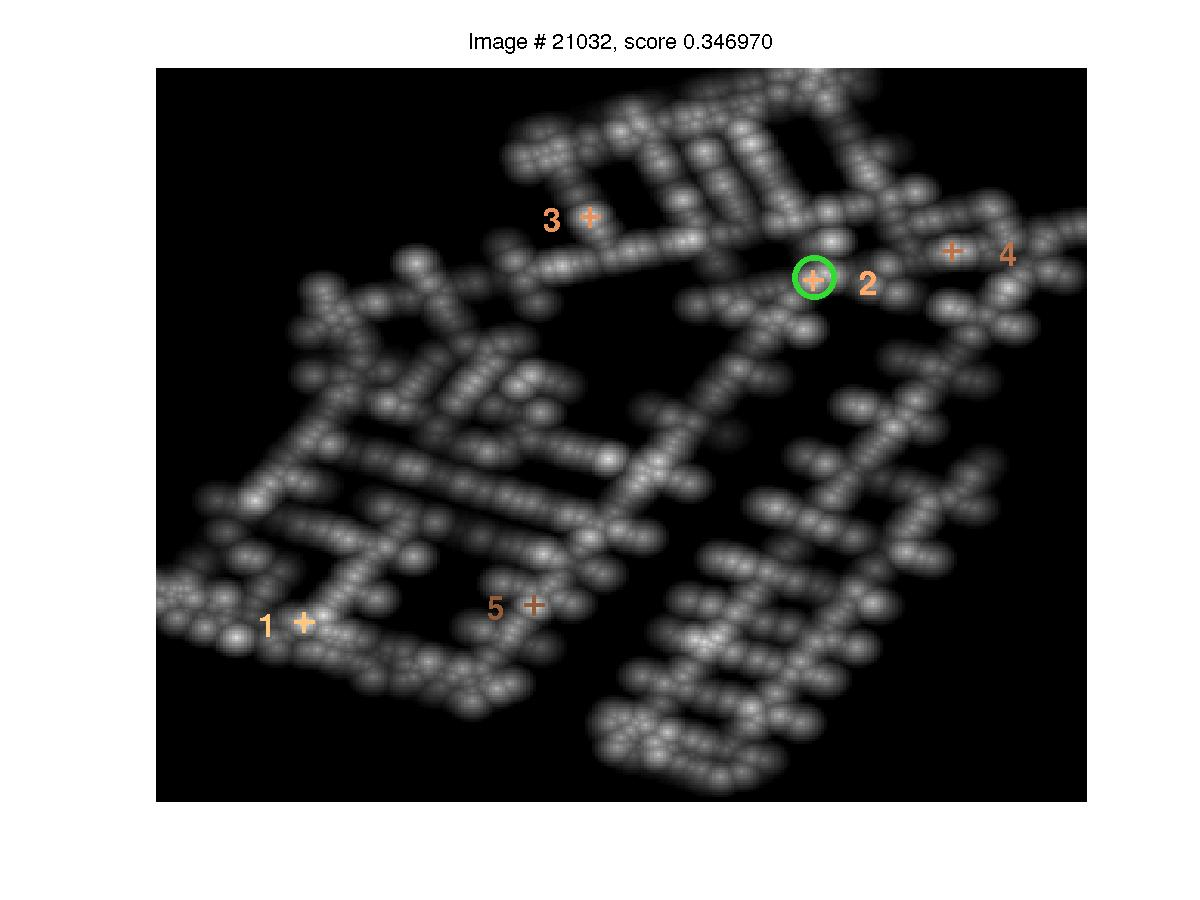
\includegraphics[trim = 55mm 40mm 55mm 25mm, clip=true,width=\linewidth]{sup1383/heatSvm.jpg}
	\end{minipage} 
	\\
	\textcolor{myWhite}{xxx}\\
	\begin{minipage}{0.45\linewidth}
		\colorbox{myGrey}{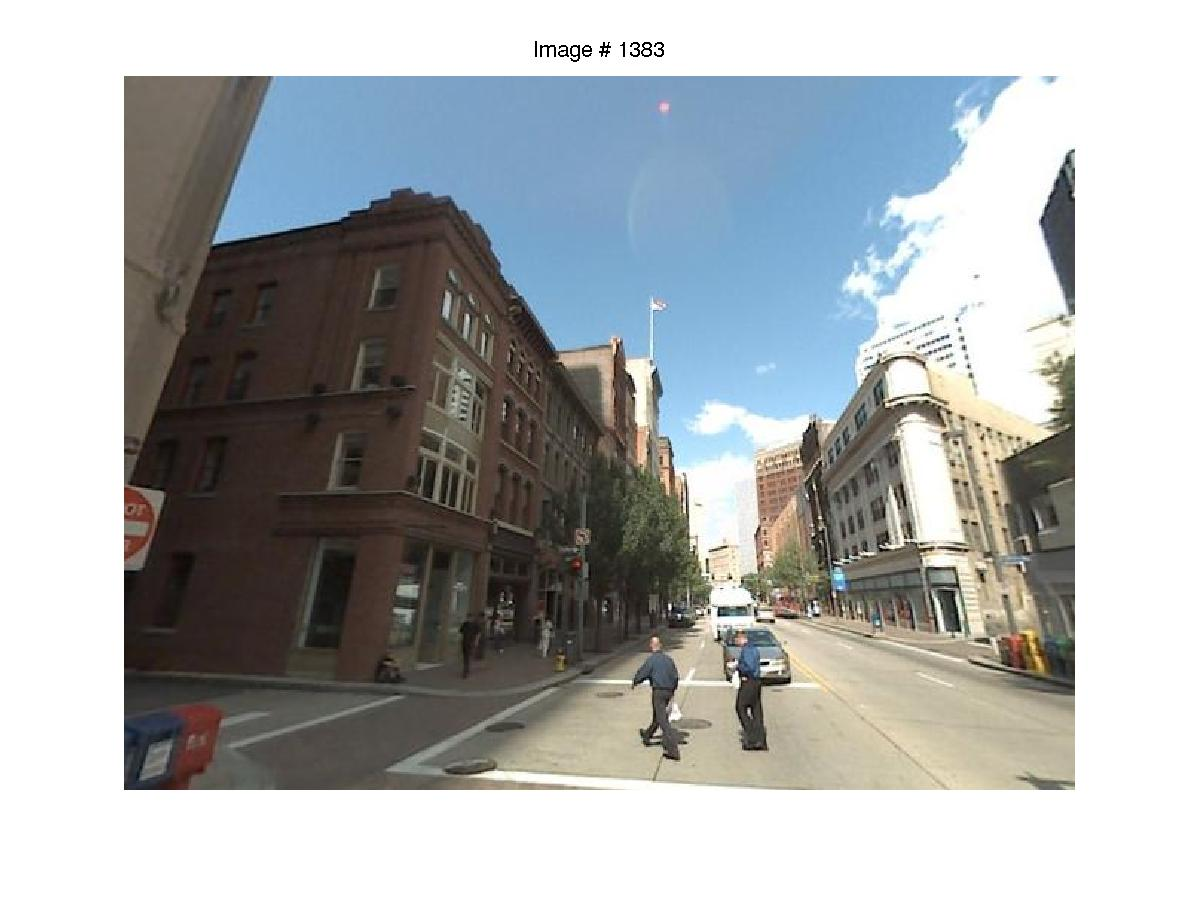
\includegraphics[trim = 55mm 40mm 55mm 30mm, clip=true,width=0.30\linewidth]{sup1383/query.jpg}}
		\colorbox{myCopper1}{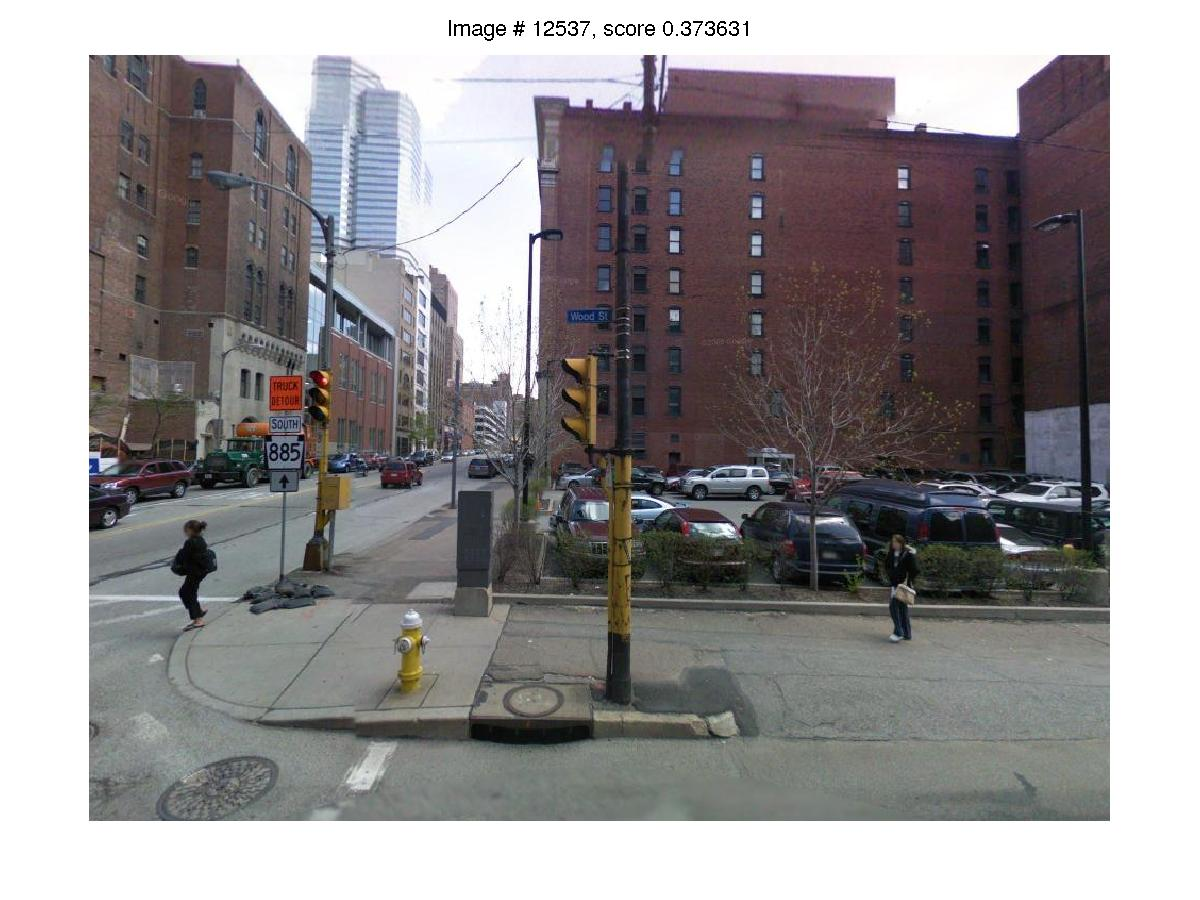
\includegraphics[trim = 55mm 40mm 55mm 30mm, clip=true,width=0.30\linewidth]{sup1383/raw01.jpg}}
		\colorbox{myCopper2}{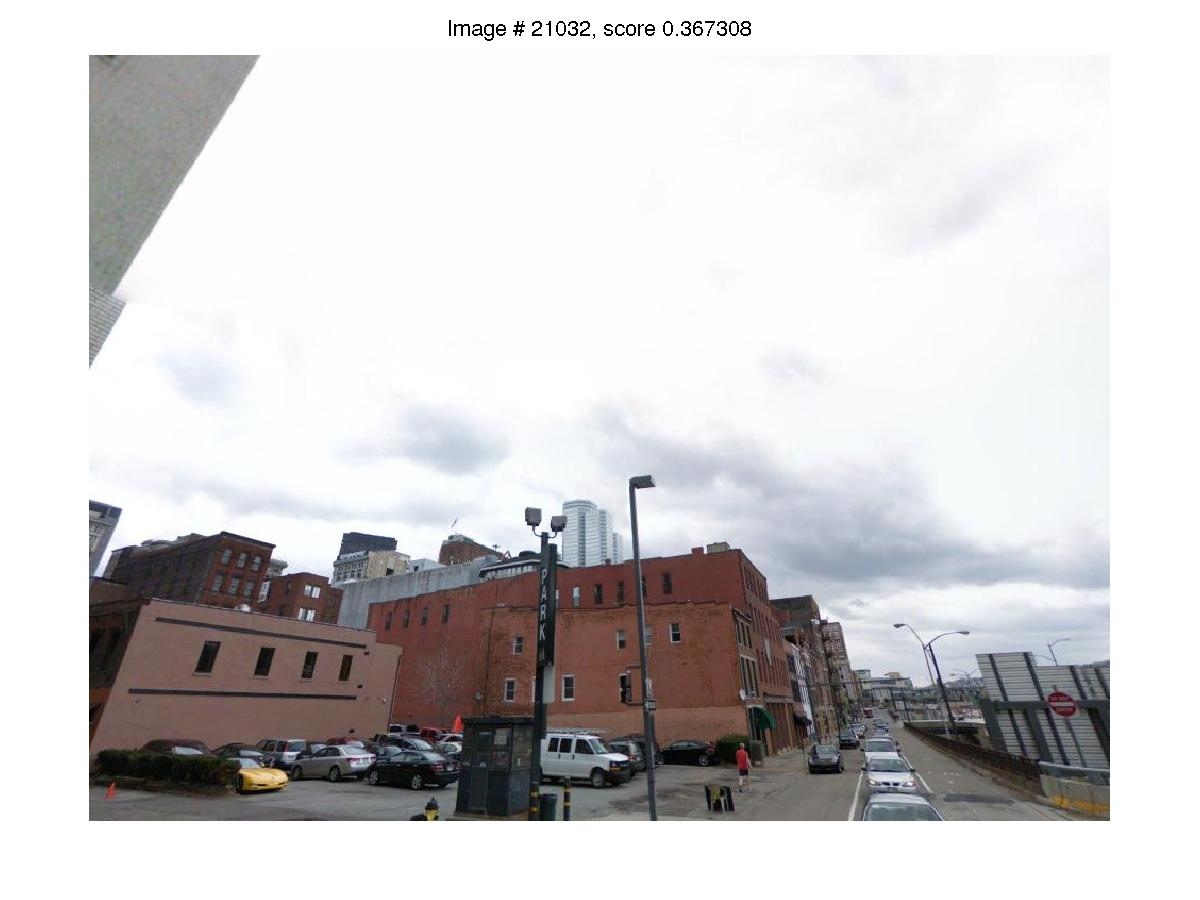
\includegraphics[trim = 55mm 40mm 55mm 30mm, clip=true,width=0.30\linewidth]{sup1383/raw02.jpg}}	\\
		\textcolor{myWhite}{xxxxxx}Query \hspace{0.25\linewidth}1. \hspace{0.25\linewidth}2. \\
		\colorbox{myCopper3}{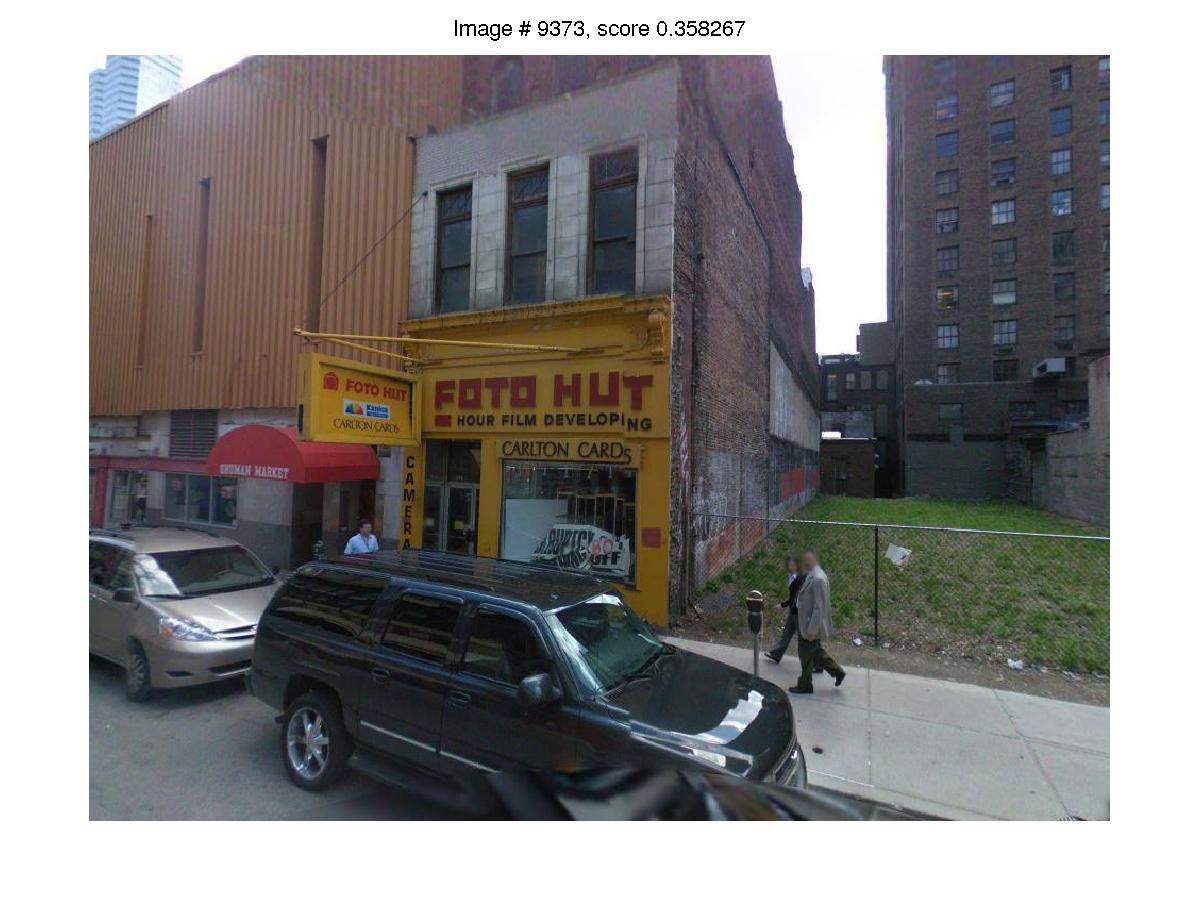
\includegraphics[trim = 55mm 40mm 55mm 30mm, clip=true,width=0.30\linewidth]{sup1383/raw03.jpg}}
		\colorbox{myCopper4}{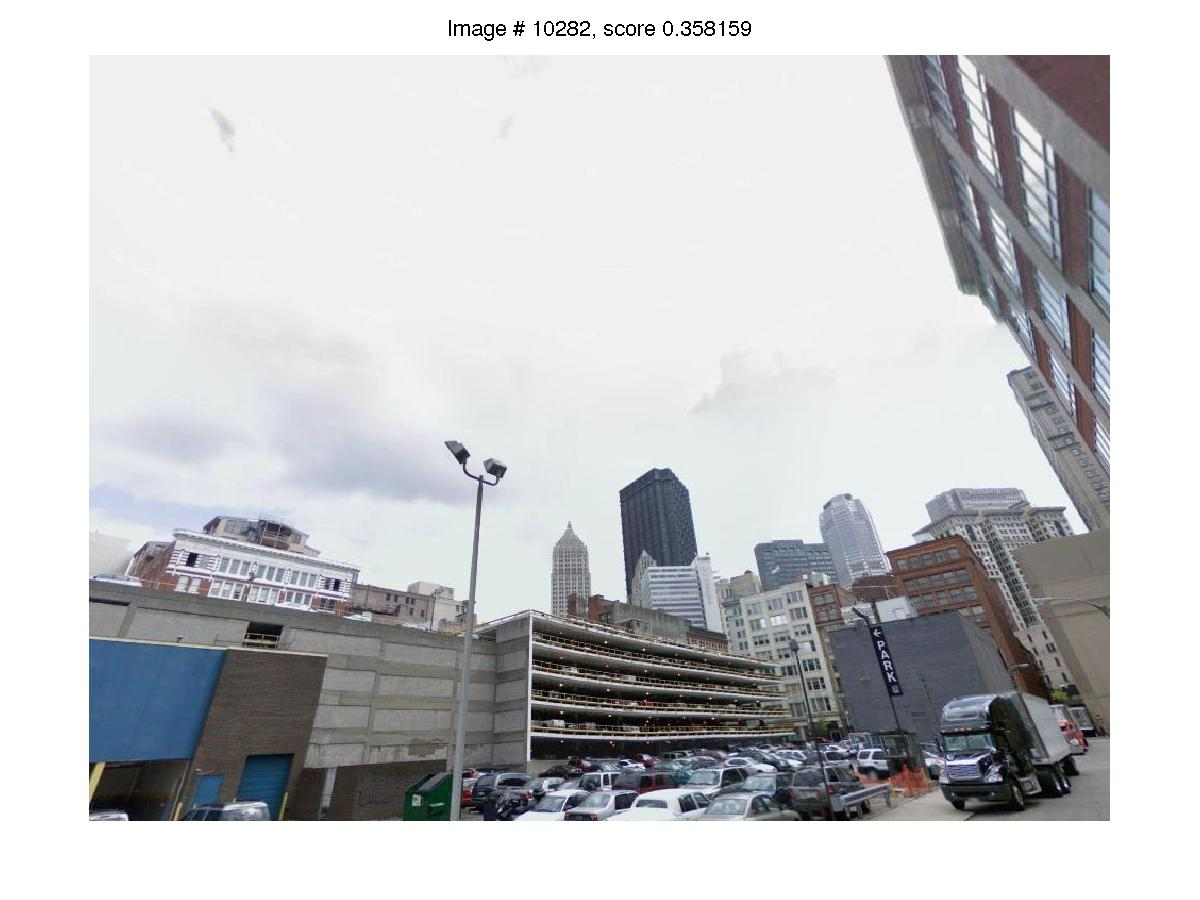
\includegraphics[trim = 55mm 40mm 55mm 30mm, clip=true,width=0.30\linewidth]{sup1383/raw04.jpg}}
		\colorbox{myCopper5}{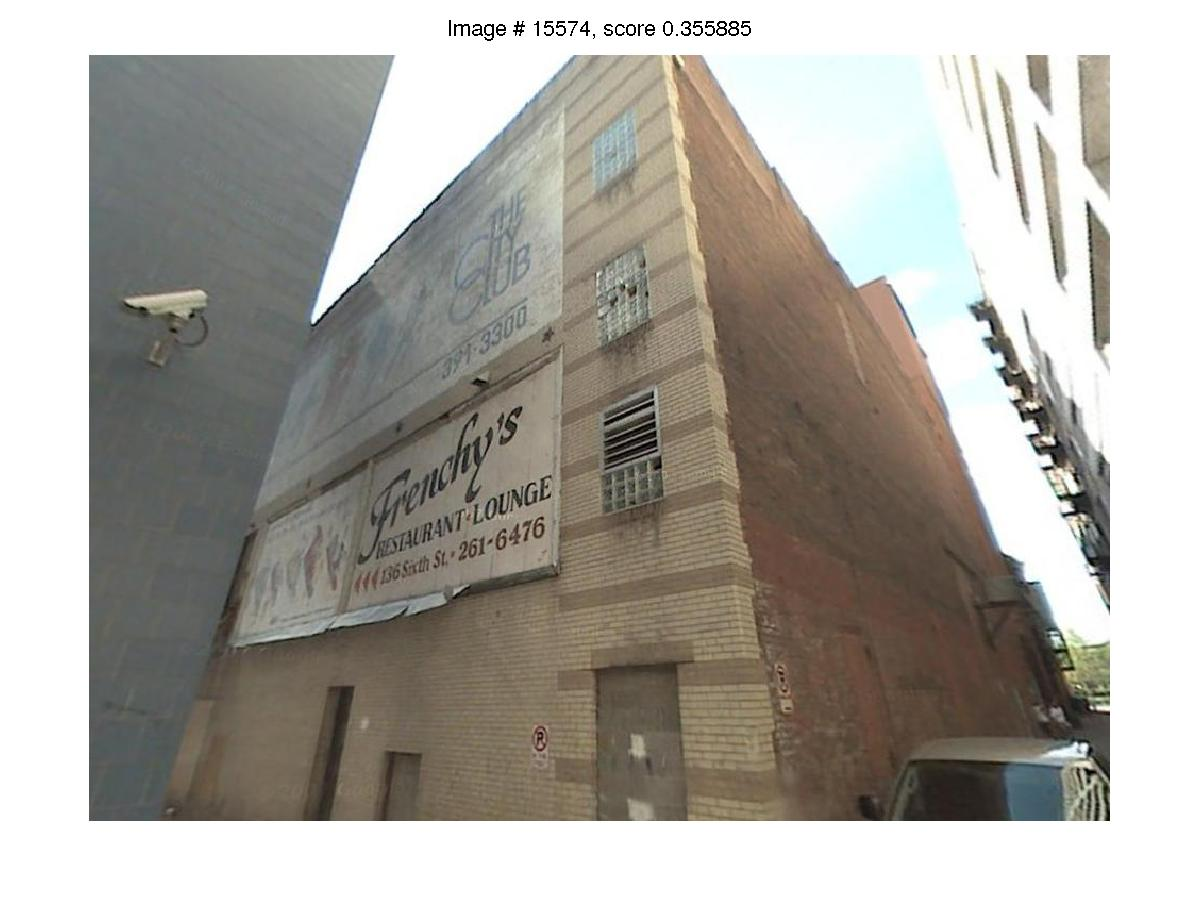
\includegraphics[trim = 55mm 40mm 55mm 30mm, clip=true,width=0.30\linewidth]{sup1383/raw05.jpg}} \\
		\textcolor{myWhite}{xxxxxx}3. \hspace{0.25\linewidth}4. \hspace{0.25\linewidth}5. \\
	\end{minipage} 
	\begin{minipage}{0.45\linewidth}
		\colorbox{myGrey}{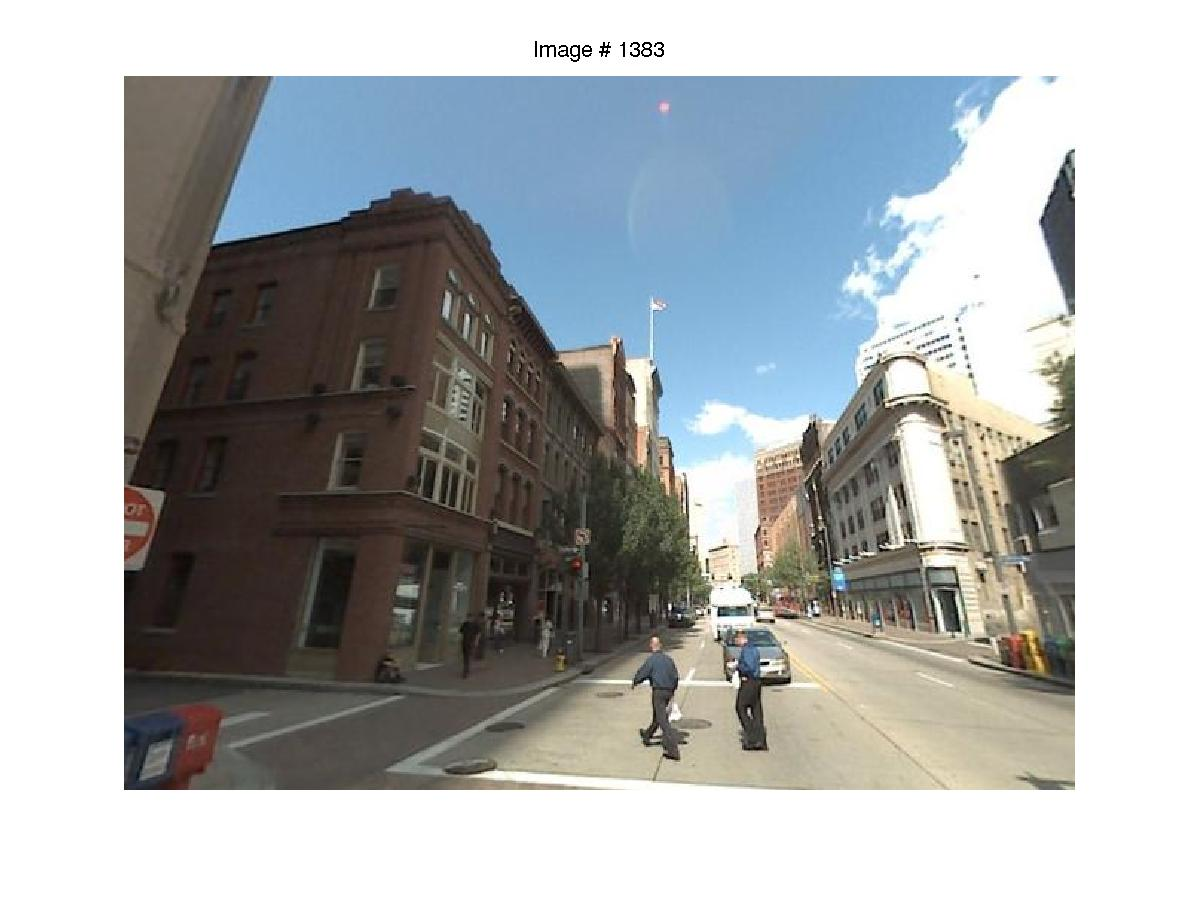
\includegraphics[trim = 55mm 40mm 55mm 30mm, clip=true,width=0.30\linewidth]{sup1383/query.jpg}}
		\colorbox{myCopper1}{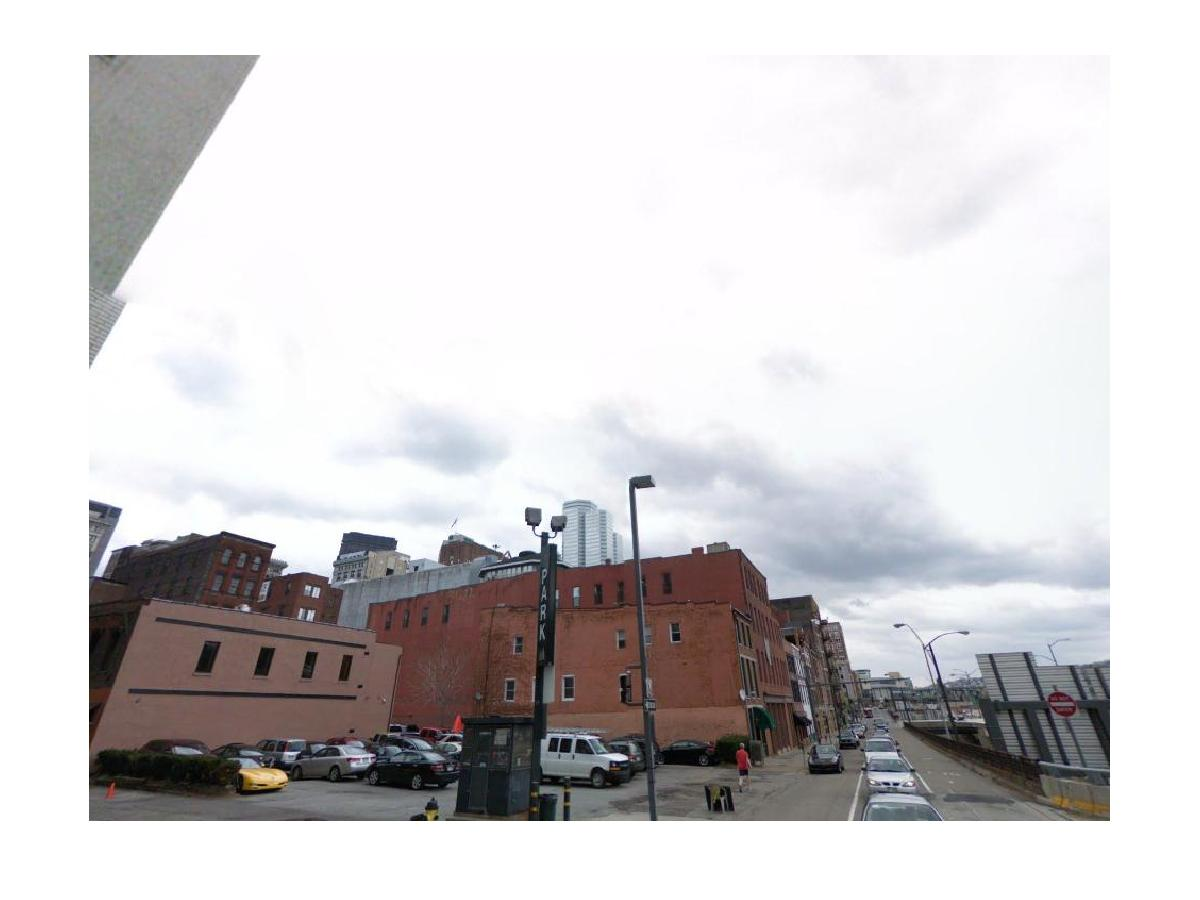
\includegraphics[trim = 55mm 40mm 55mm 30mm, clip=true,width=0.30\linewidth]{sup1383/svm01.jpg}}
		\colorbox{myGreen}{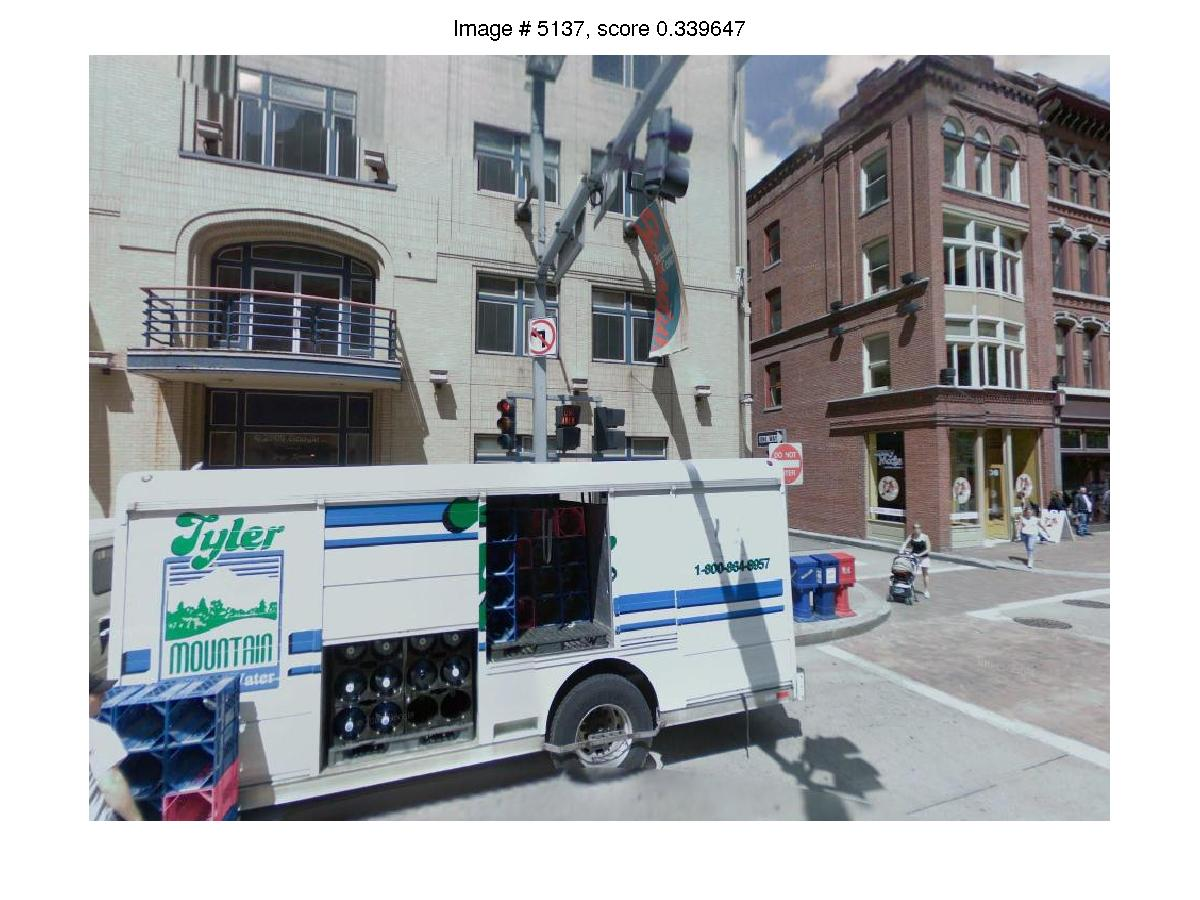
\includegraphics[trim = 55mm 40mm 55mm 30mm, clip=true,width=0.30\linewidth]{sup1383/svm02.jpg}}	\\
		\textcolor{myWhite}{xxxxxx}Query \hspace{0.25\linewidth}1. \hspace{0.25\linewidth}2. \\
		\colorbox{myCopper3}{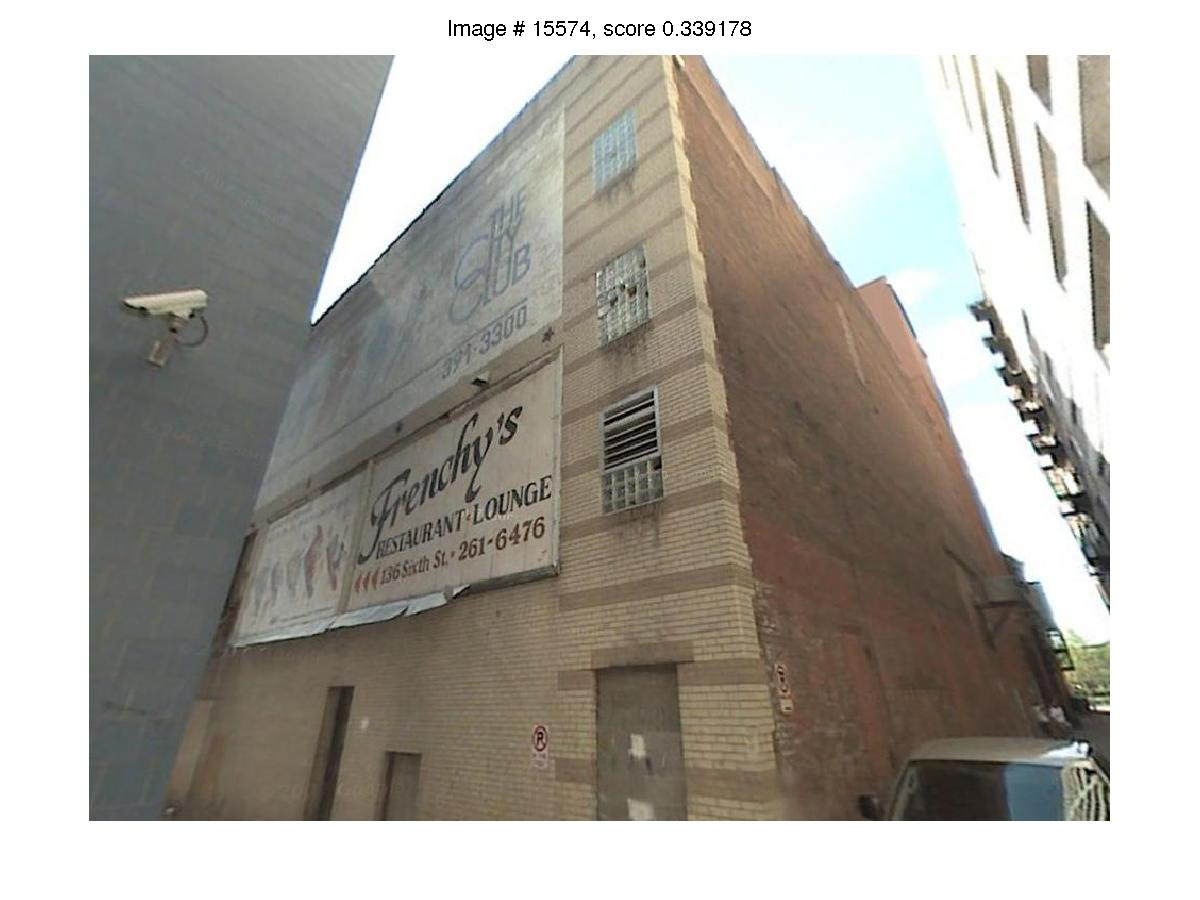
\includegraphics[trim = 55mm 40mm 55mm 30mm, clip=true,width=0.30\linewidth]{sup1383/svm03.jpg}}
		\colorbox{myCopper4}{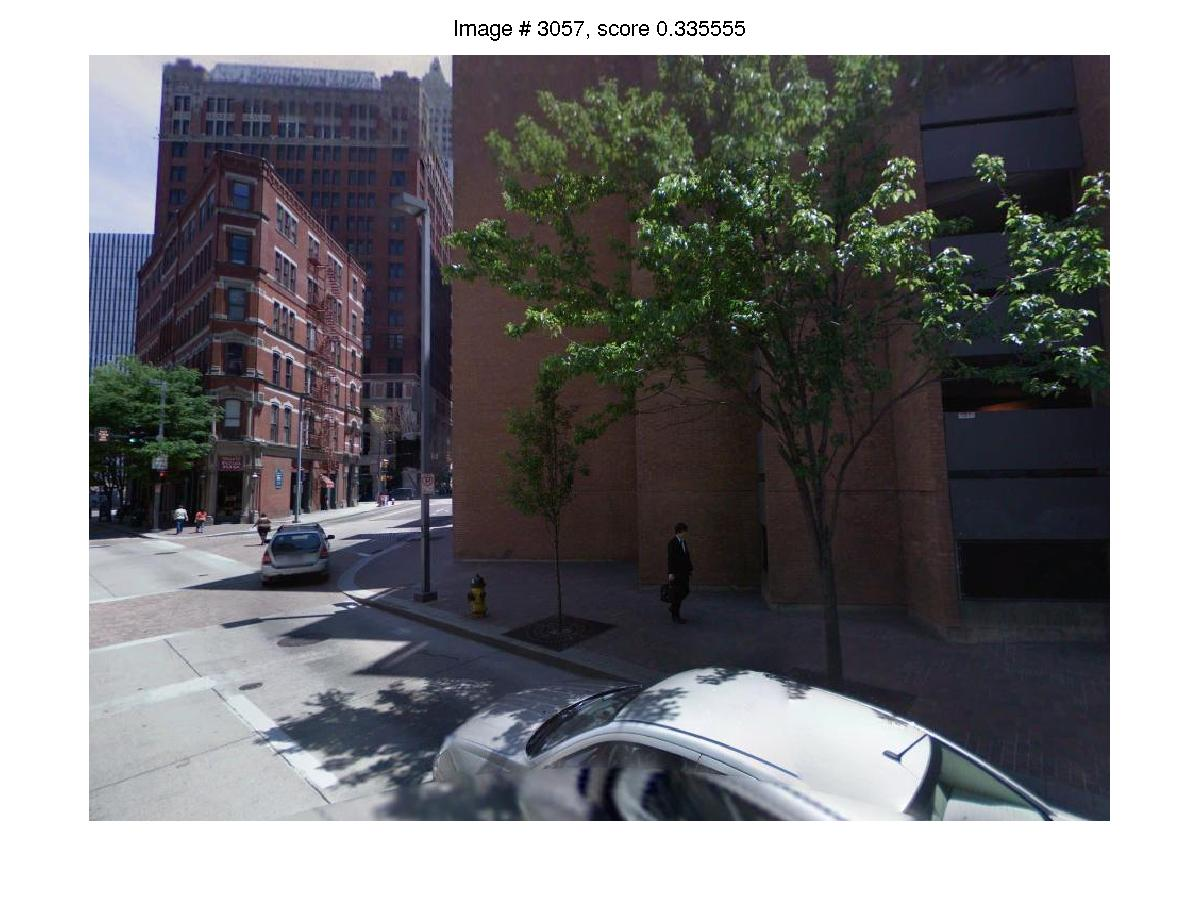
\includegraphics[trim = 55mm 40mm 55mm 30mm, clip=true,width=0.30\linewidth]{sup1383/svm04.jpg}}
		\colorbox{myCopper5}{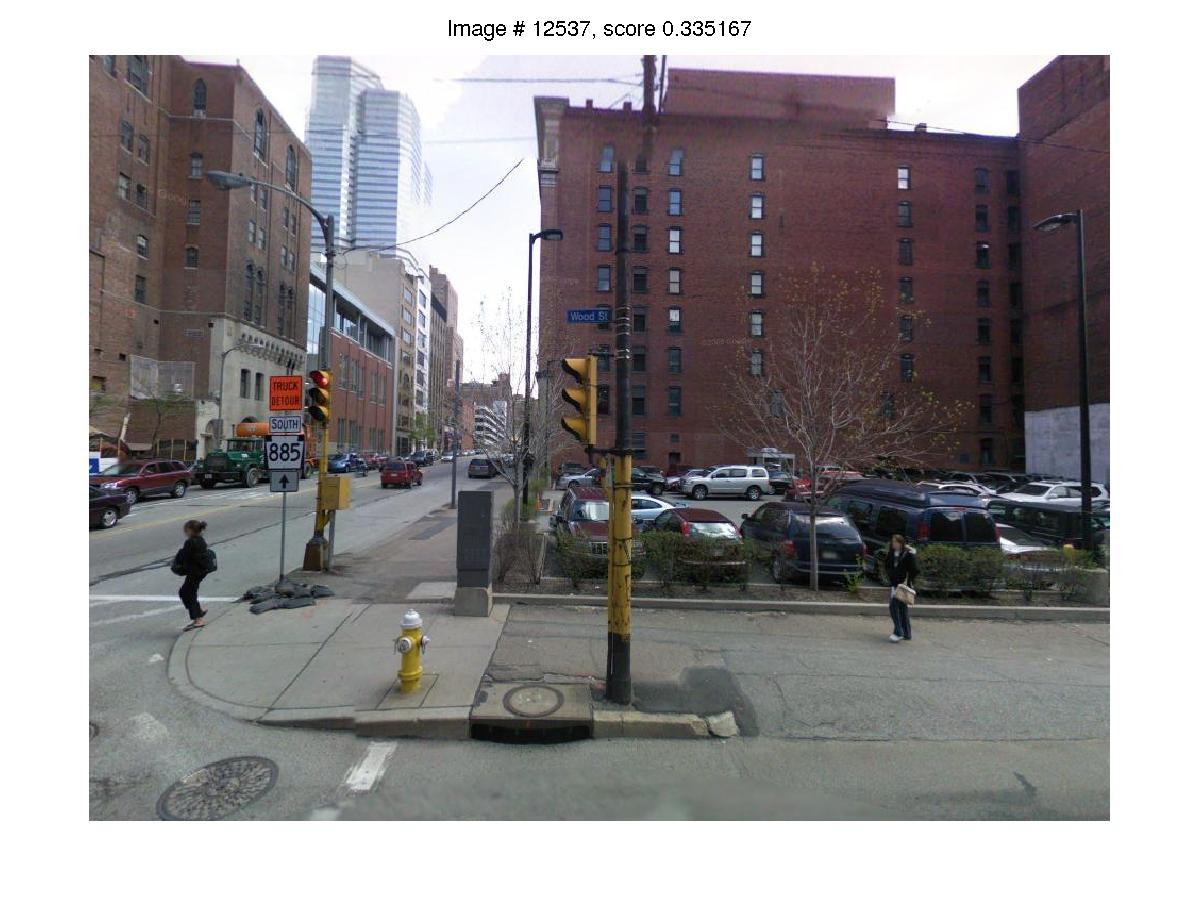
\includegraphics[trim = 55mm 40mm 55mm 30mm, clip=true,width=0.30\linewidth]{sup1383/svm05.jpg}}  \\
		\textcolor{myWhite}{xxxxxx}3. \hspace{0.25\linewidth}4. \hspace{0.25\linewidth}5. \\
	\end{minipage}
	%\caption{Example sup1383} 
%	\caption{ \textbf{Response of Fisher vector accross the databse images.}
%		\emph{Top row:} The heatmaps show a distribution of the Fisher vector (FV) similarity score with a given query image. A location of the query image is shown by green circle, top 5 strongest peaks are denoted by a cross marker along with its rank. \emph{Bottom row:} The query image is shown in a gray box and top five database images corresponding to the top 5 strongest peaks in the map. The correct match is denoted by green bounding box.
%		Each FV score votes into a max-pooling accumulation array that corresponds to a GPS location of the database images.
%		\emph{Left} column shows results for raw FV baseline without any learning while \emph{right} column displays results for FV obtained by proposed method (e-SVM FV). Notice that e-SVM FV descriptor suppress the peaks that are far from the query image which results into a change of ranking.
%		}
	\caption{{\bf Top:} 
	Matching scores for the same query image shown across the entire database on the map. Brighter pixels indicate higher (better) scores. The ground truth position of the query image is shown as a green circle. The map also shows the position and rank of the top five matches. {\bf Bottom:} The top five matches for the same query before (left) and after (right) learning.
	Note that the proposed method (right) correctly localized the query image within the top five matched locations. 
	The matched image is shown in green. 
	{\bf Animation:} The animation shows the score map for the same query with the raw FV descriptors and the proposed learnt compact descriptor. Note that the learnt descriptors better discriminate different places on the map and hence some of the high scoring false positive peaks for this query are suppressed.
%	Note that the proposed method suppresses the high-scores far from the query image, which results in a change of ranking.}
}
%	
%	\textbf{Response of Fisher vector accross the databse images.}
%		\emph{Top row:} The heatmaps show a distribution of the Fisher vector (FV) similarity score with a given query image. A location of the query image is shown by green circle, top 5 strongest peaks are denoted by a cross marker along with its rank. \emph{Bottom row:} The query image is shown in a gray box and top five database images corresponding to the top 5 strongest peaks in the map. The correct match is denoted by green bounding box.
%		Each FV score votes into a max-pooling accumulation array that corresponds to a GPS location of the database images.
%		\emph{Left} column shows results for raw FV baseline without any learning while \emph{right} column displays results for FV obtained by proposed method (e-SVM FV). Notice that e-SVM FV descriptor suppress the peaks that are far from the query image which results into a change of ranking.
%}
\end{figure}


\begin{figure}
	\begin{minipage}{0.45\linewidth}
		\center
		(raw FV128 baseline) \\
		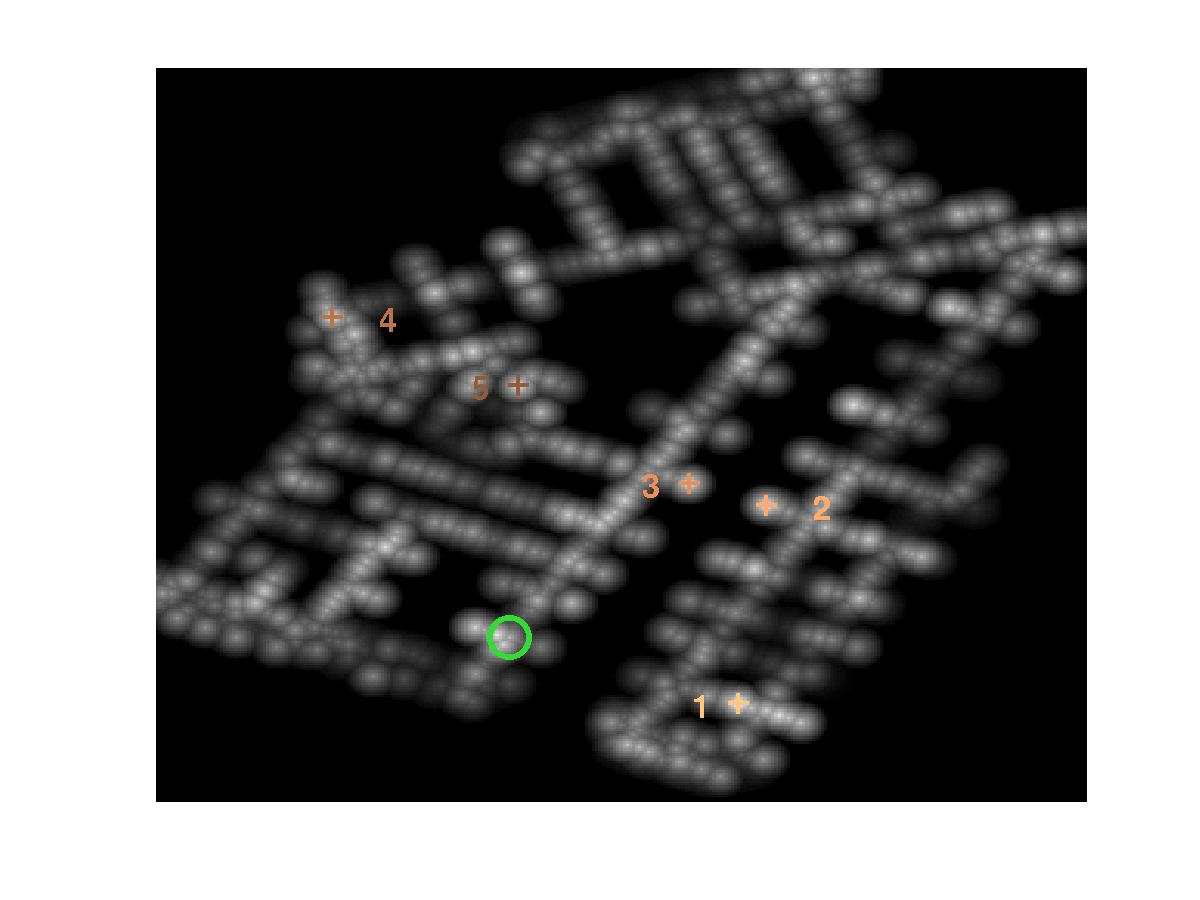
\includegraphics[trim = 55mm 40mm 55mm 25mm, clip=true,width=\linewidth]{sup1666/heatRaw.jpg}
	\end{minipage} 
	\begin{minipage}{0.45\linewidth}
		\center
		(e-SVM FV128) \\
		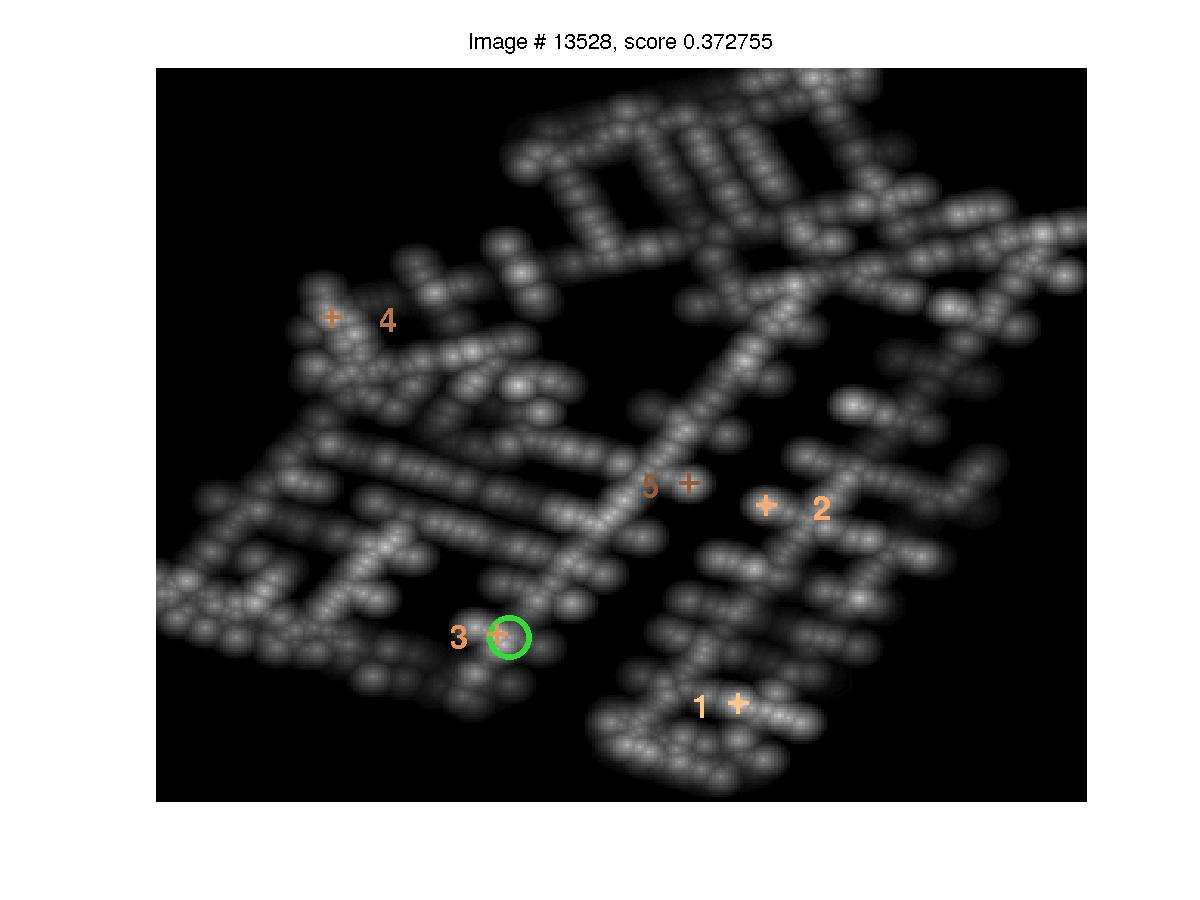
\includegraphics[trim = 55mm 40mm 55mm 25mm, clip=true,width=\linewidth]{sup1666/heatSvm.jpg}
	\end{minipage} 
	\\
	\textcolor{myWhite}{xxx}\\
	\begin{minipage}{0.45\linewidth}
		\colorbox{myGrey}{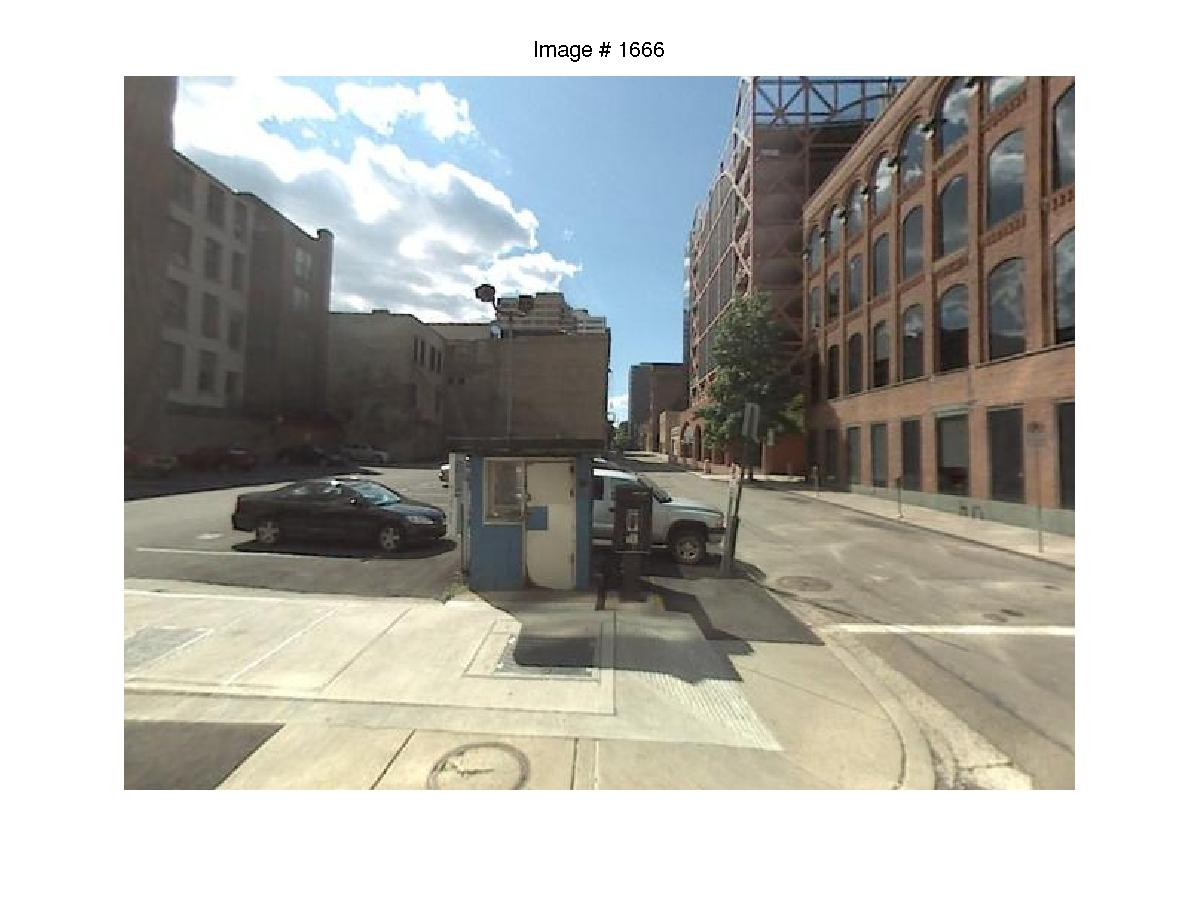
\includegraphics[trim = 55mm 40mm 55mm 30mm, clip=true,width=0.30\linewidth]{sup1666/query.jpg}}
		\colorbox{myCopper1}{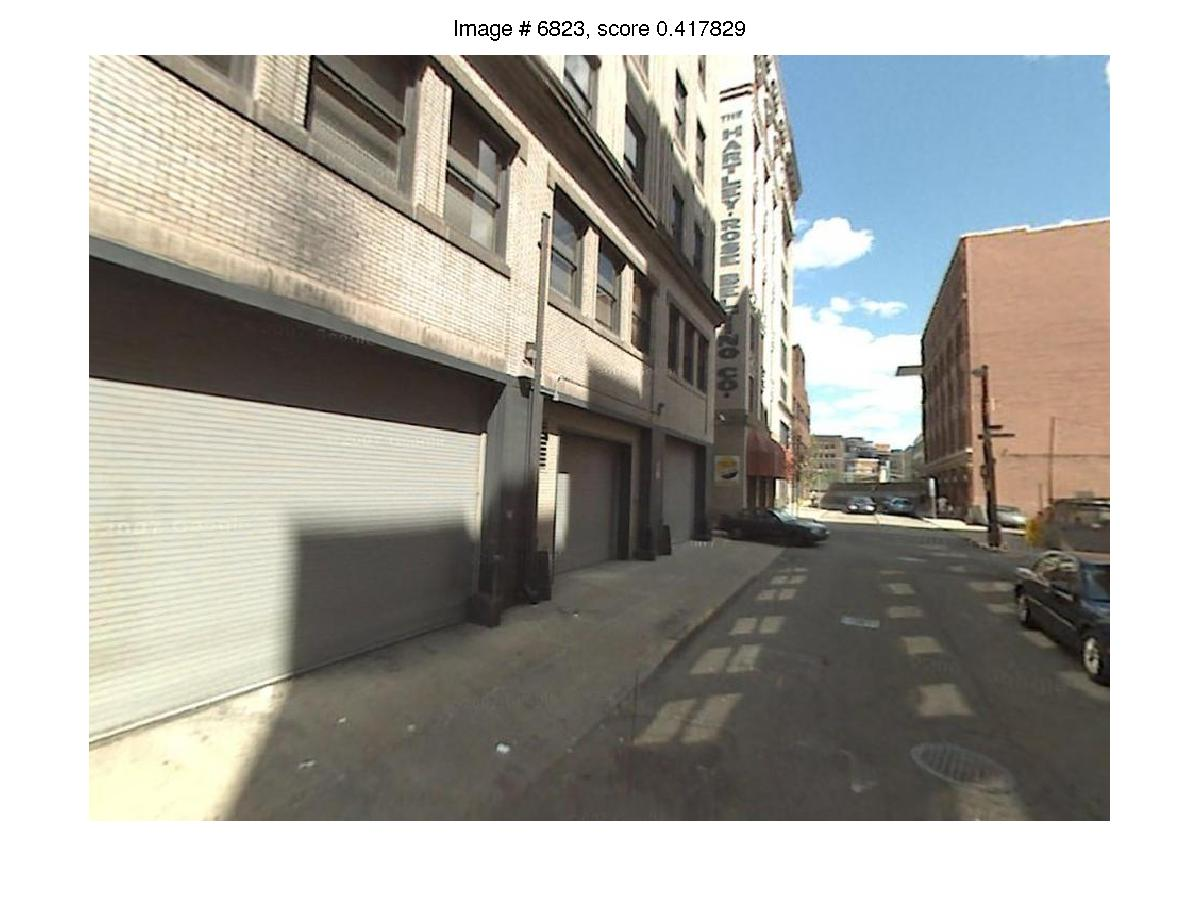
\includegraphics[trim = 55mm 40mm 55mm 30mm, clip=true,width=0.30\linewidth]{sup1666/raw01.jpg}}
		\colorbox{myCopper2}{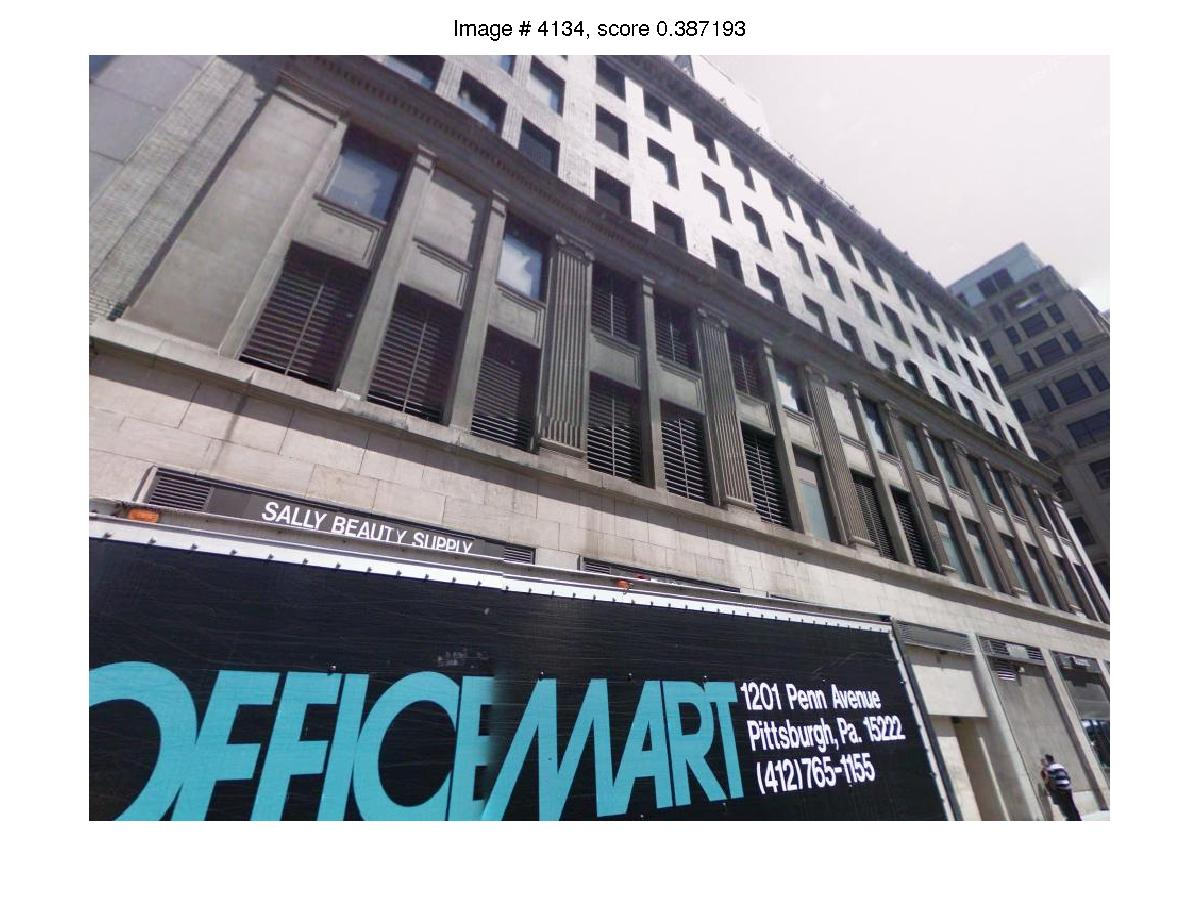
\includegraphics[trim = 55mm 40mm 55mm 30mm, clip=true,width=0.30\linewidth]{sup1666/raw02.jpg}}	\\
		\textcolor{myWhite}{xxxxxx}Query \hspace{0.25\linewidth}1. \hspace{0.25\linewidth}2. \\
		\colorbox{myCopper3}{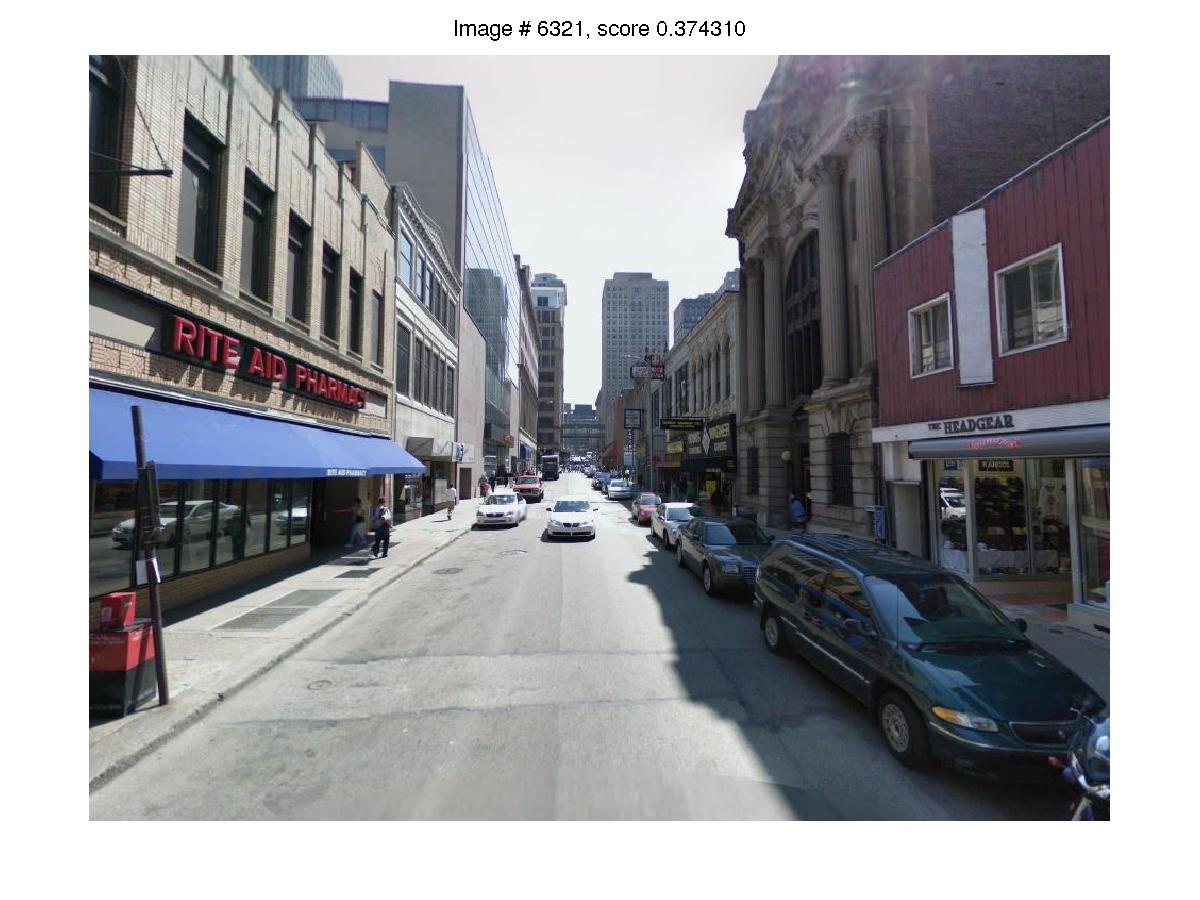
\includegraphics[trim = 55mm 40mm 55mm 30mm, clip=true,width=0.30\linewidth]{sup1666/raw03.jpg}}
		\colorbox{myCopper4}{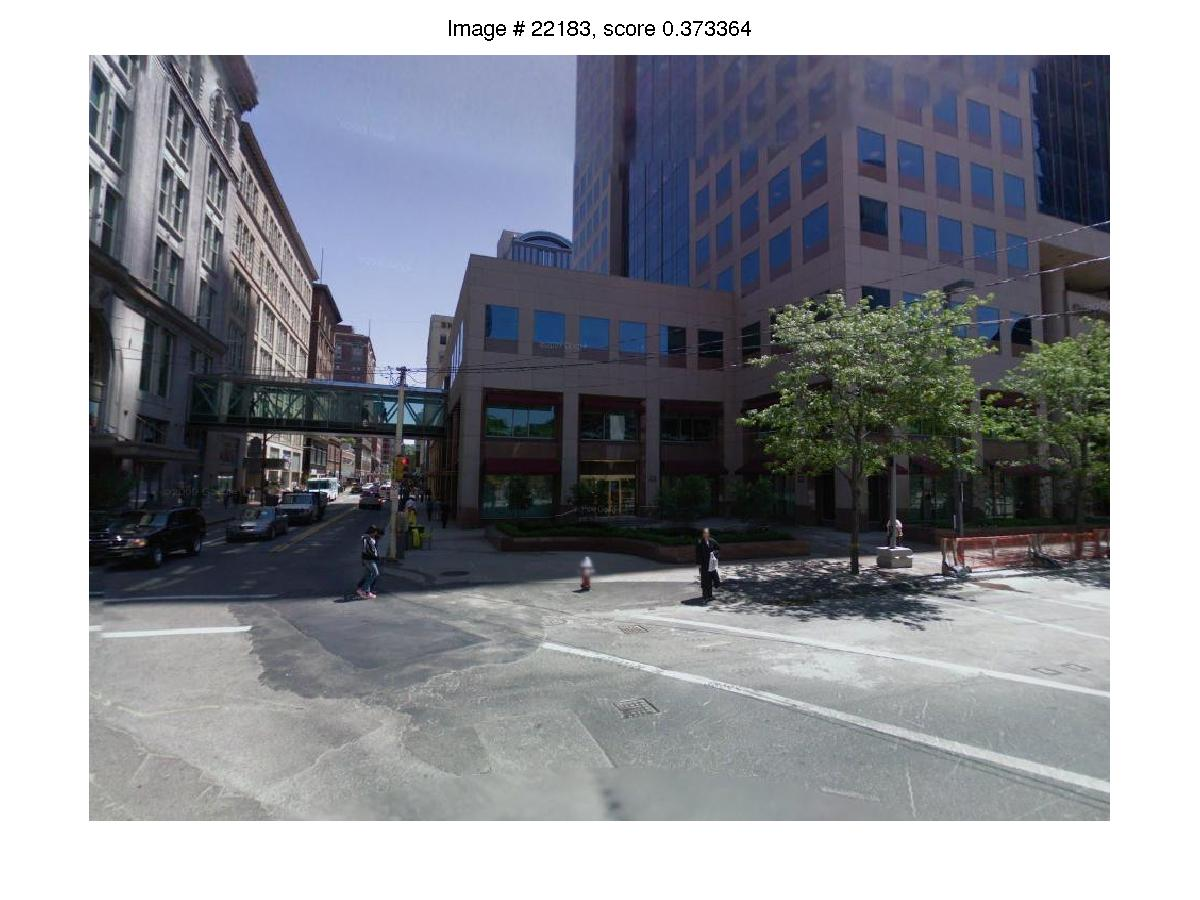
\includegraphics[trim = 55mm 40mm 55mm 30mm, clip=true,width=0.30\linewidth]{sup1666/raw04.jpg}}
		\colorbox{myCopper5}{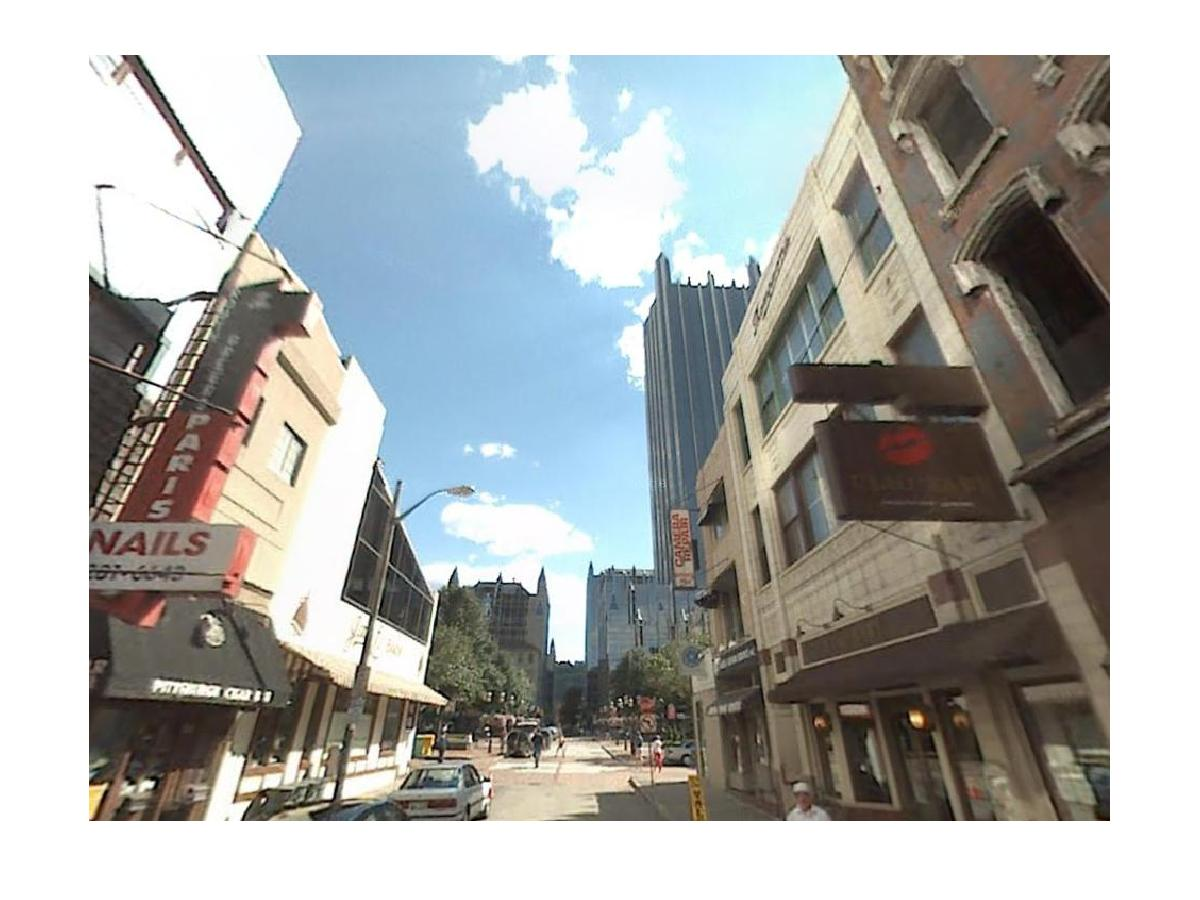
\includegraphics[trim = 55mm 40mm 55mm 30mm, clip=true,width=0.30\linewidth]{sup1666/raw05.jpg}} \\
		\textcolor{myWhite}{xxxxxx}3. \hspace{0.25\linewidth}4. \hspace{0.25\linewidth}5. \\
	\end{minipage} 
	\begin{minipage}{0.45\linewidth}
		\colorbox{myGrey}{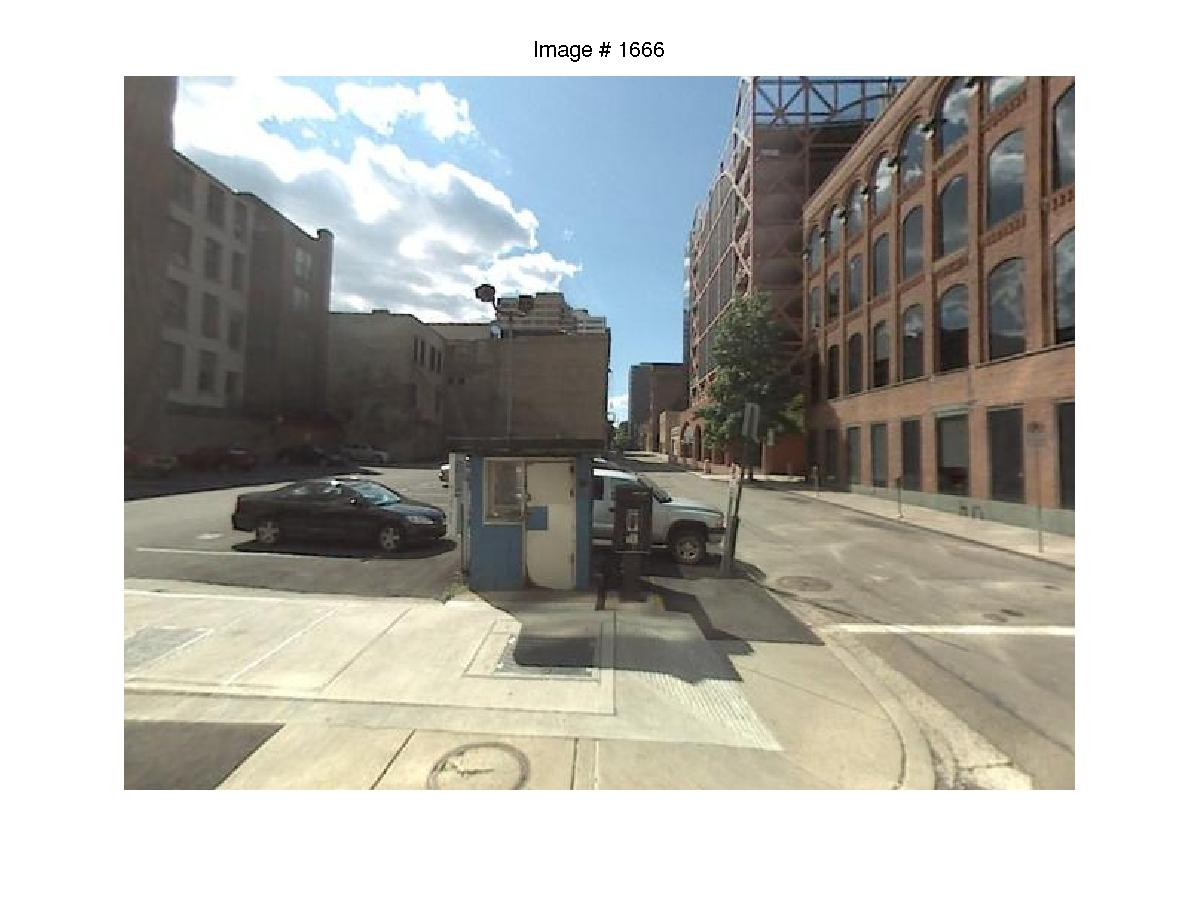
\includegraphics[trim = 55mm 40mm 55mm 30mm, clip=true,width=0.30\linewidth]{sup1666/query.jpg}}
		\colorbox{myCopper1}{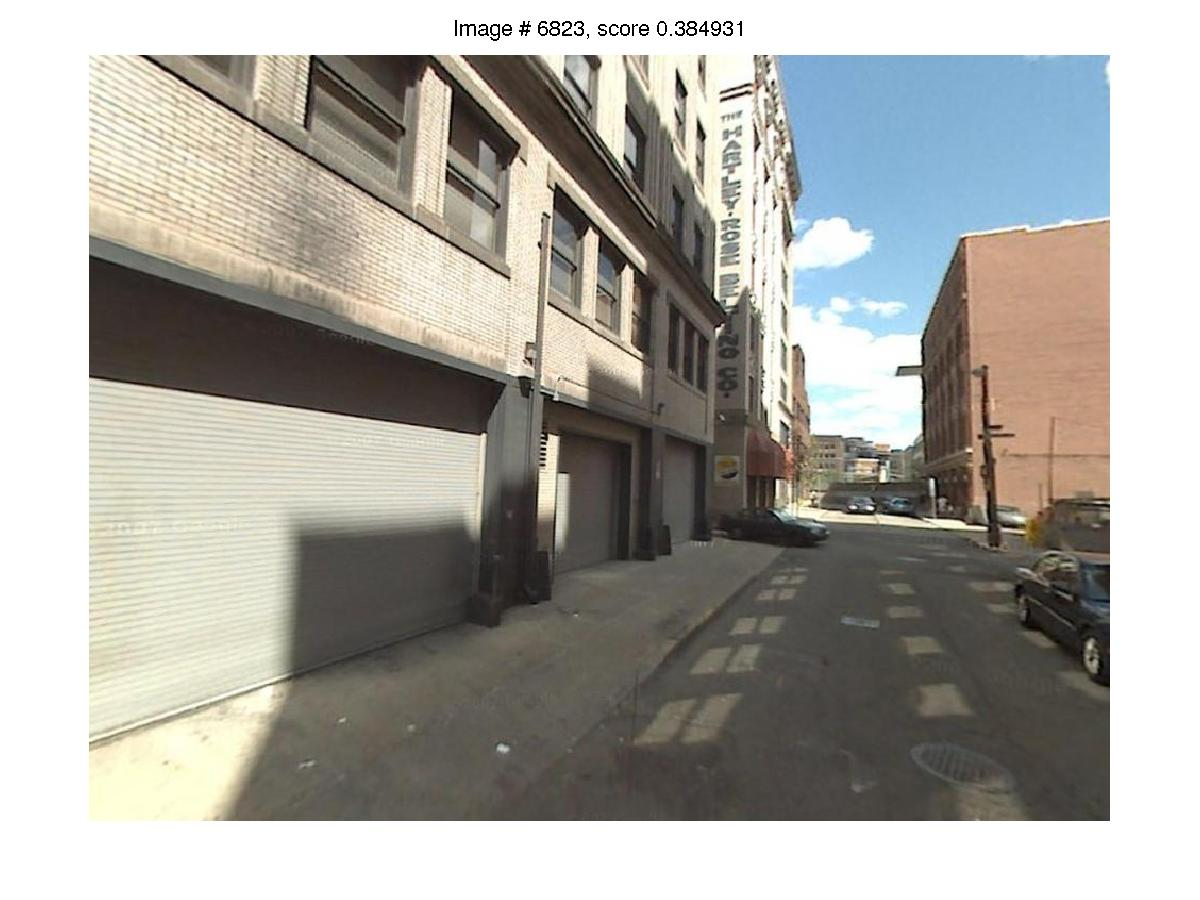
\includegraphics[trim = 55mm 40mm 55mm 30mm, clip=true,width=0.30\linewidth]{sup1666/svm01.jpg}}
		\colorbox{myCopper2}{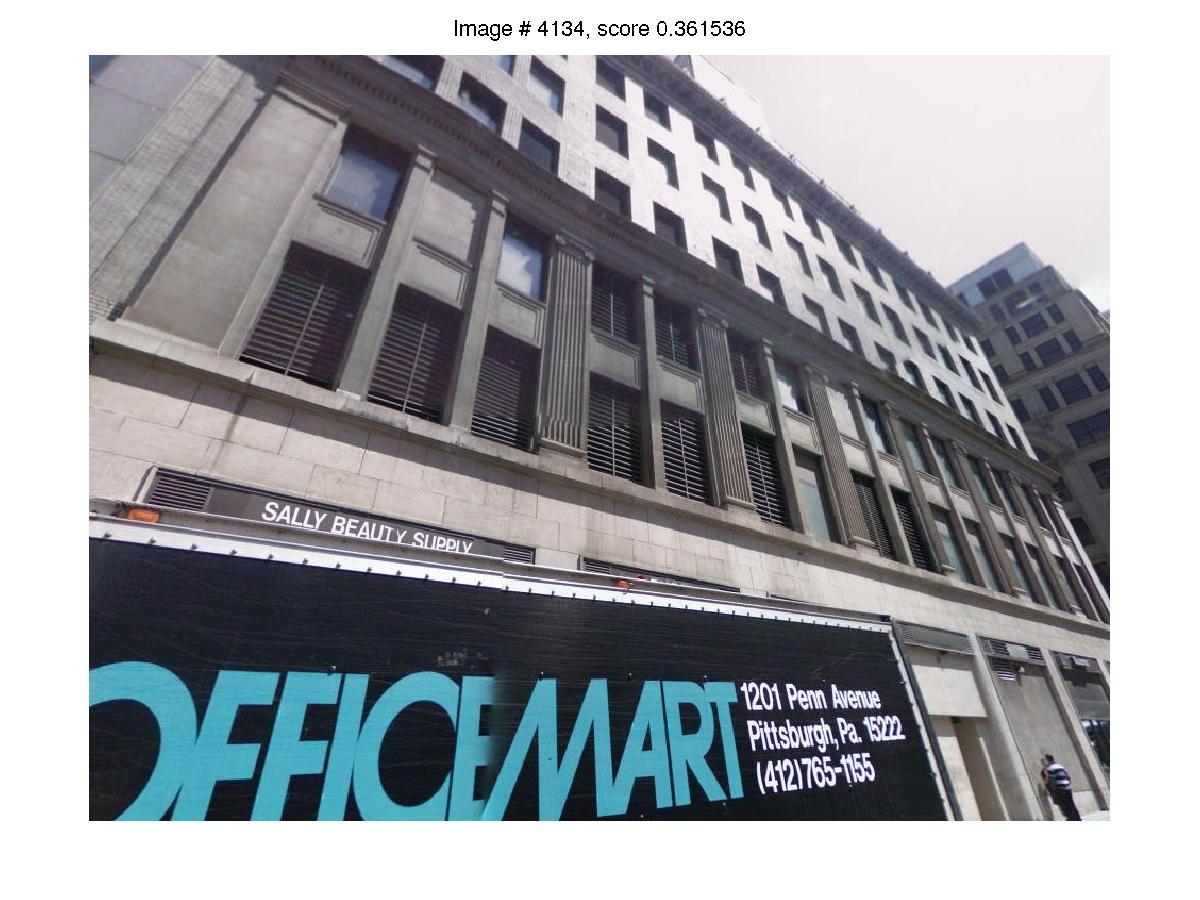
\includegraphics[trim = 55mm 40mm 55mm 30mm, clip=true,width=0.30\linewidth]{sup1666/svm02.jpg}}	\\
		\textcolor{myWhite}{xxxxxx}Query \hspace{0.25\linewidth}1. \hspace{0.25\linewidth}2. \\
		\colorbox{myGreen}{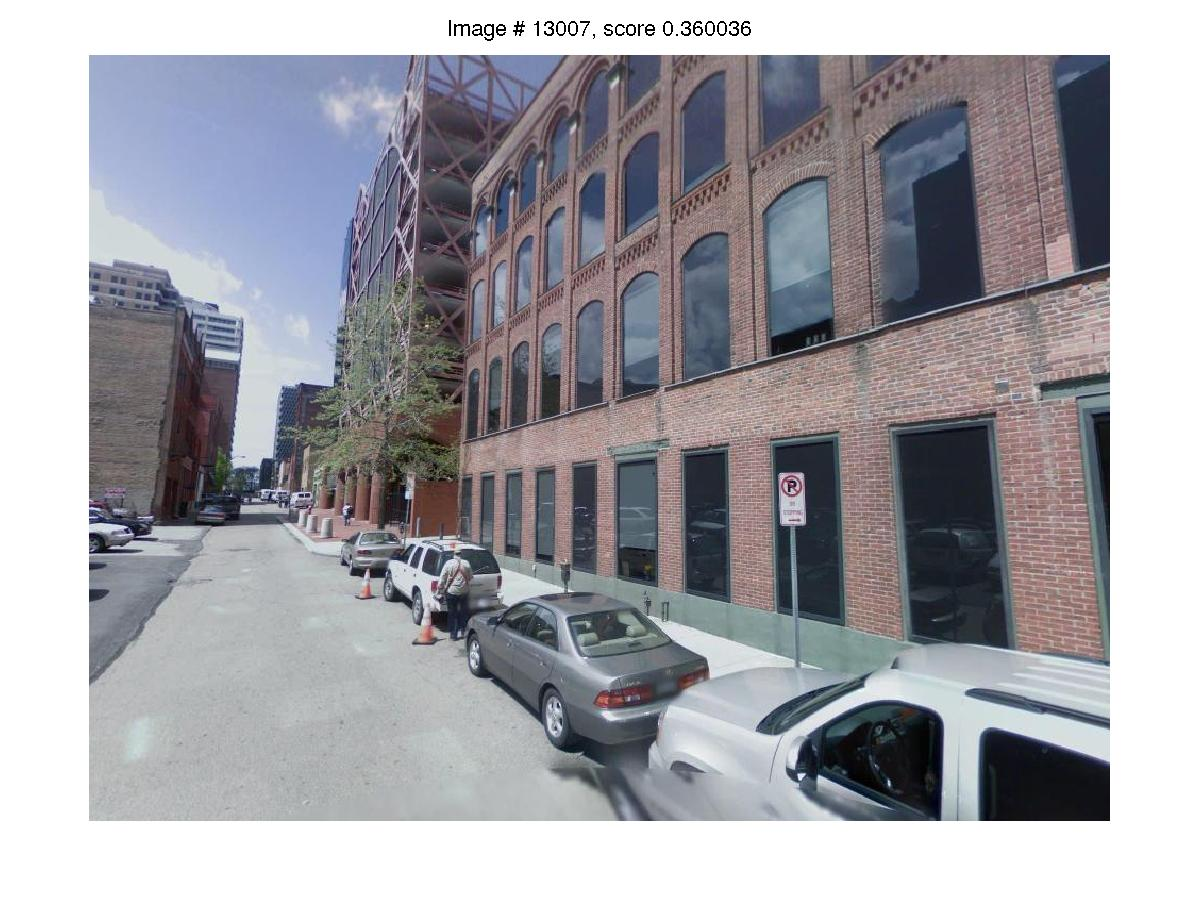
\includegraphics[trim = 55mm 40mm 55mm 30mm, clip=true,width=0.30\linewidth]{sup1666/svm03.jpg}}
		\colorbox{myCopper4}{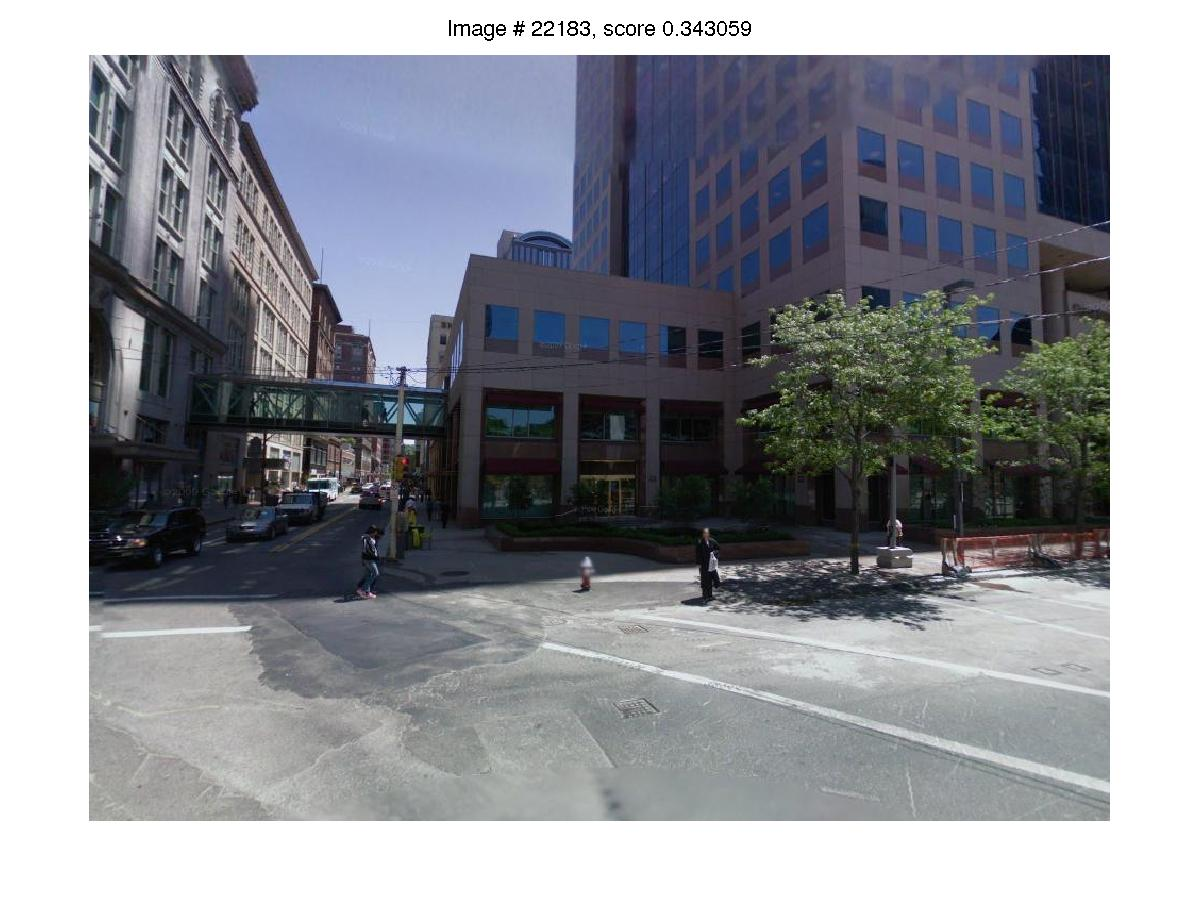
\includegraphics[trim = 55mm 40mm 55mm 30mm, clip=true,width=0.30\linewidth]{sup1666/svm04.jpg}}
		\colorbox{myCopper5}{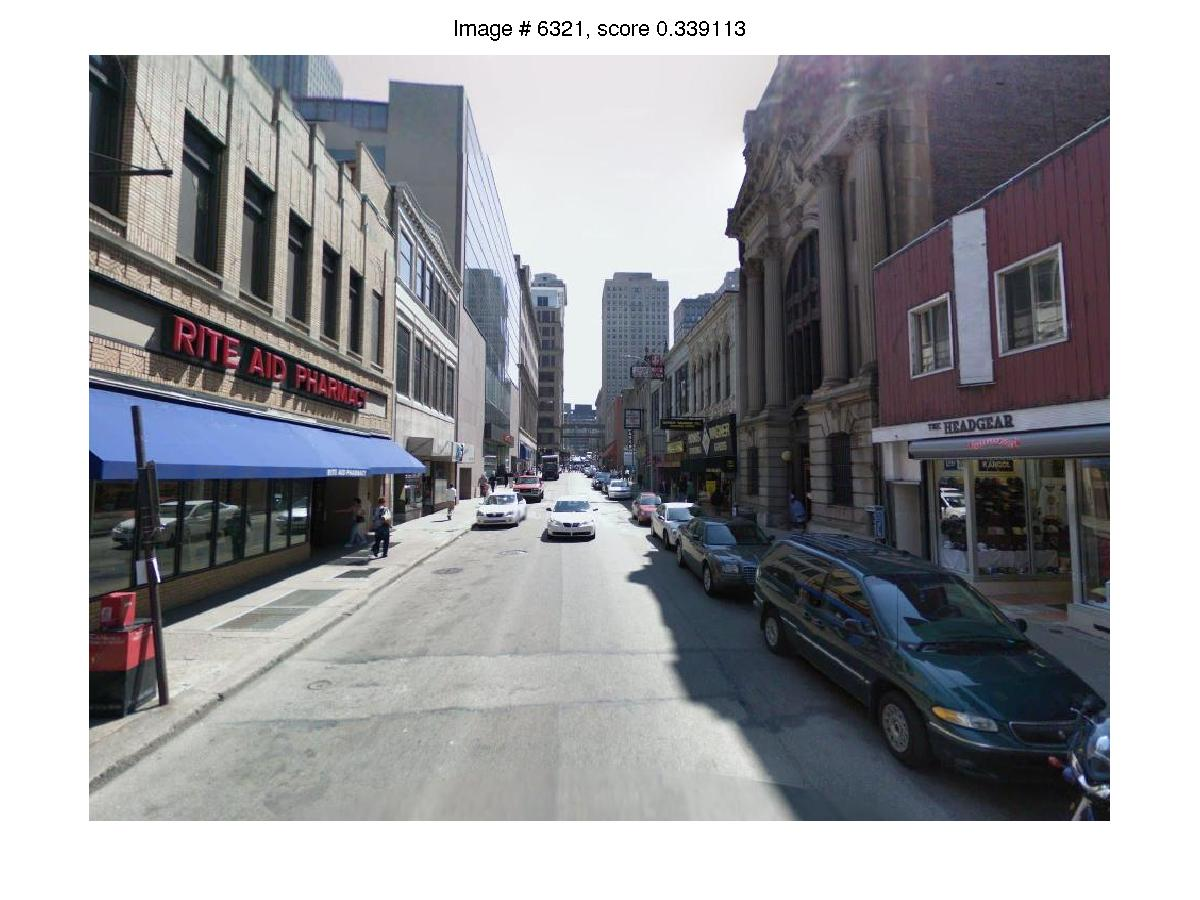
\includegraphics[trim = 55mm 40mm 55mm 30mm, clip=true,width=0.30\linewidth]{sup1666/svm05.jpg}}  \\
		\textcolor{myWhite}{xxxxxx}3. \hspace{0.25\linewidth}4. \hspace{0.25\linewidth}5. \\
	\end{minipage}
	%\caption{Example sup1666} 
\end{figure}


\begin{figure}
	\begin{minipage}{0.45\linewidth}
		\center
		(raw FV128 baseline) \\
		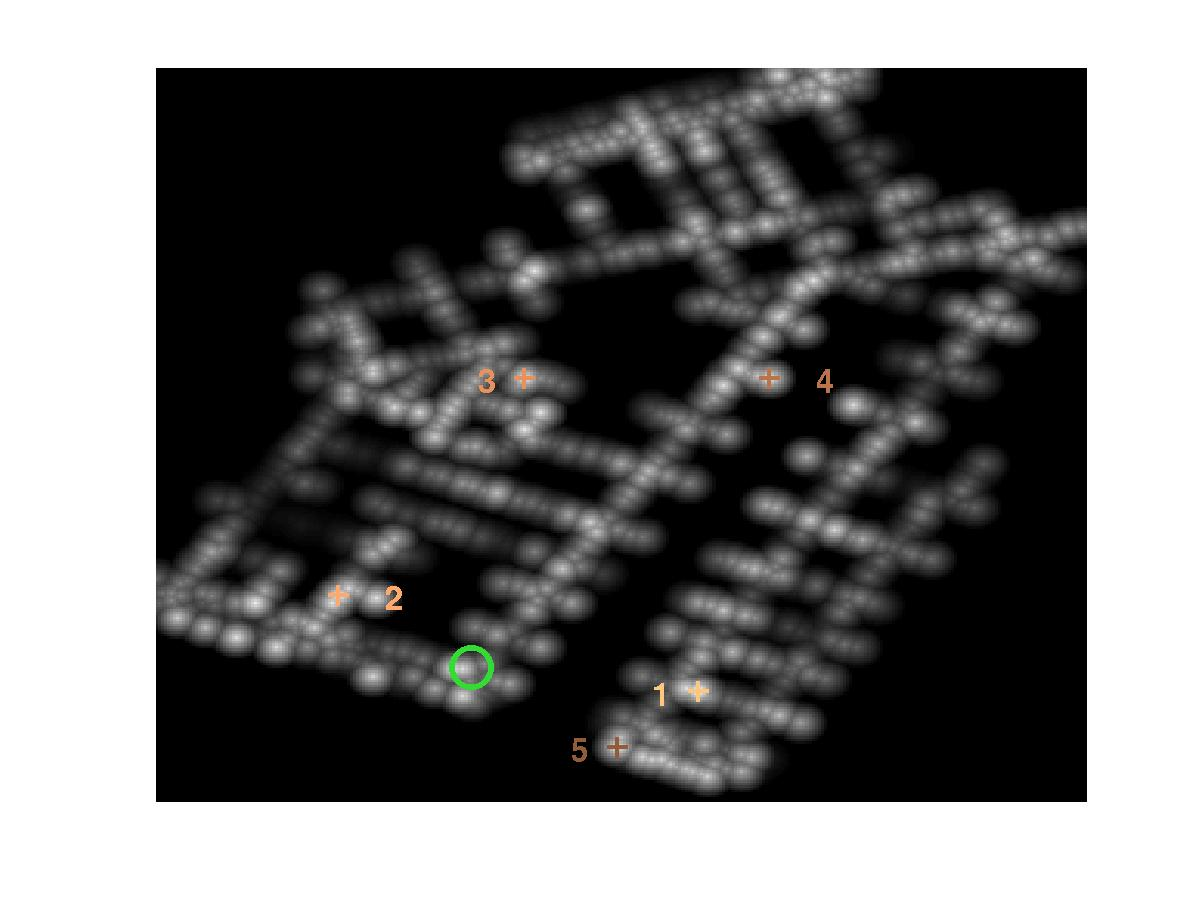
\includegraphics[trim = 55mm 40mm 55mm 25mm, clip=true,width=\linewidth]{sup1693/heatRaw.jpg}
	\end{minipage} 
	\begin{minipage}{0.45\linewidth}
		\center
		(e-SVM FV128) \\
		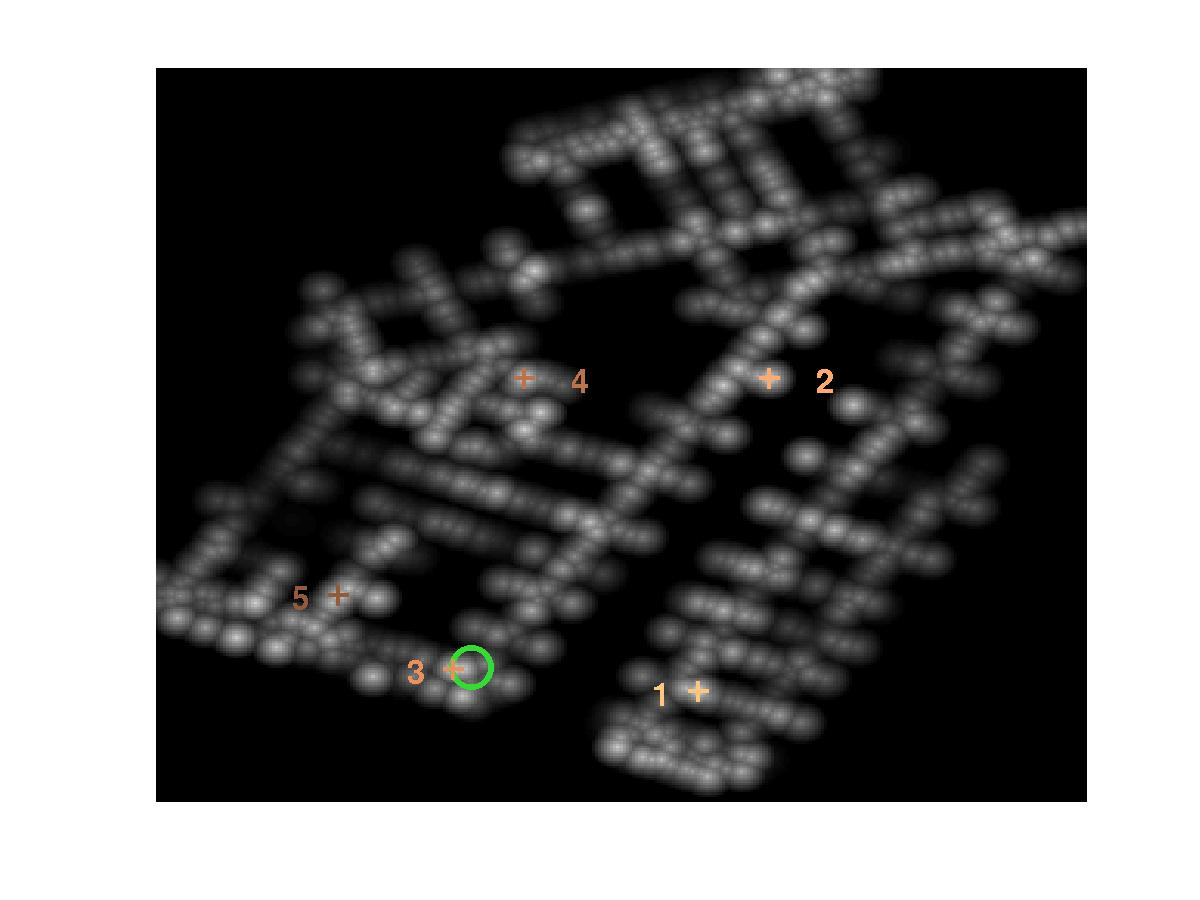
\includegraphics[trim = 55mm 40mm 55mm 25mm, clip=true,width=\linewidth]{sup1693/heatSvm.jpg}
	\end{minipage} 
	\\
	\textcolor{myWhite}{xxx}\\
	\begin{minipage}{0.45\linewidth}
		\colorbox{myGrey}{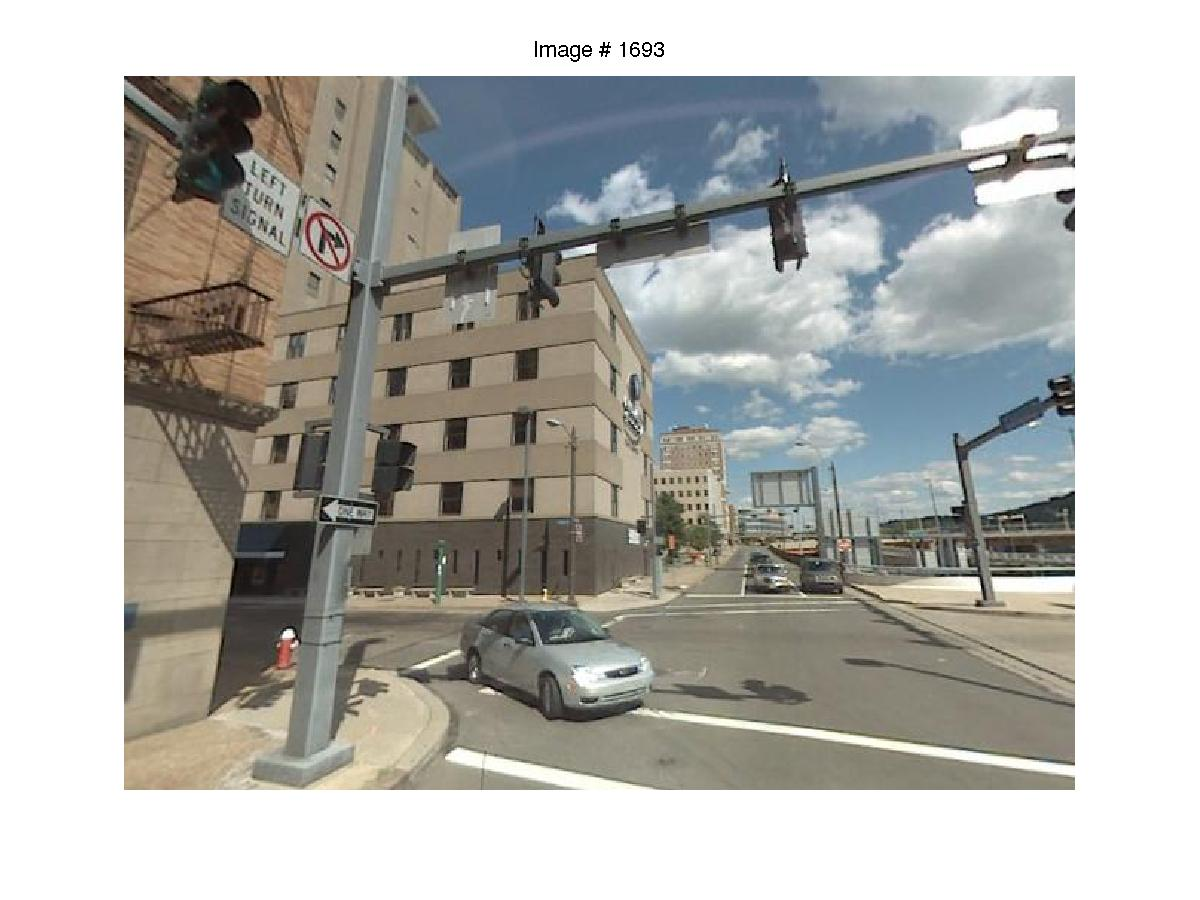
\includegraphics[trim = 55mm 40mm 55mm 30mm, clip=true,width=0.30\linewidth]{sup1693/query.jpg}}
		\colorbox{myCopper1}{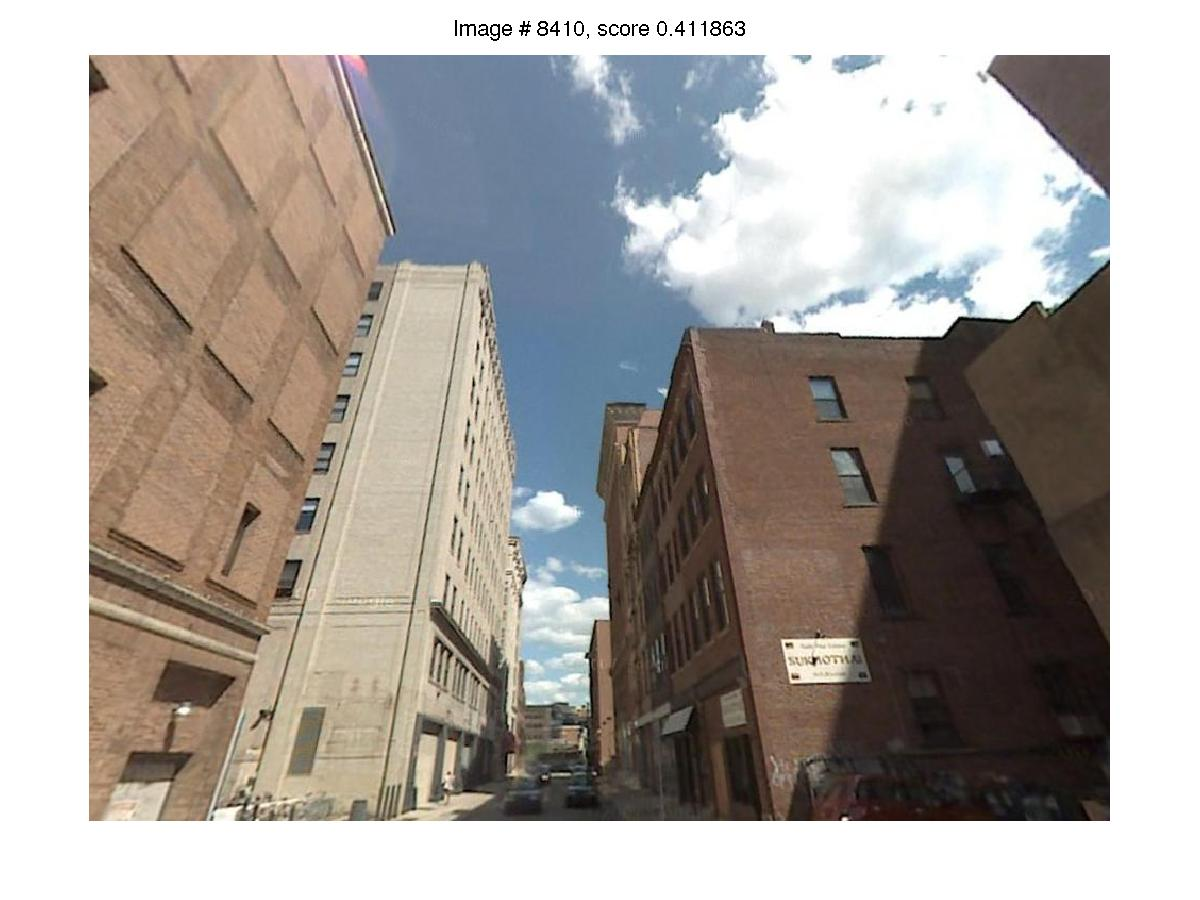
\includegraphics[trim = 55mm 40mm 55mm 30mm, clip=true,width=0.30\linewidth]{sup1693/raw01.jpg}}
		\colorbox{myCopper2}{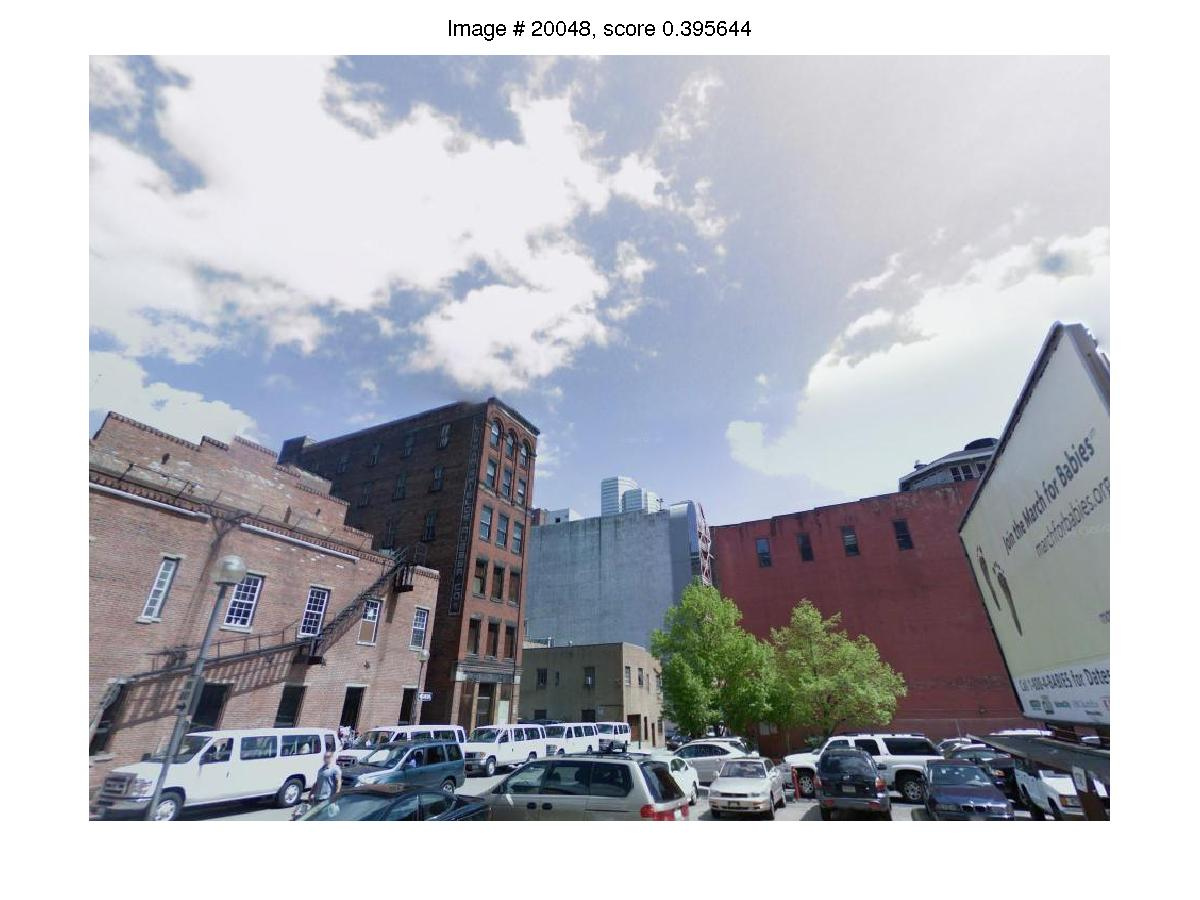
\includegraphics[trim = 55mm 40mm 55mm 30mm, clip=true,width=0.30\linewidth]{sup1693/raw02.jpg}}	\\
		\textcolor{myWhite}{xxxxxx}Query \hspace{0.25\linewidth}1. \hspace{0.25\linewidth}2. \\
		\colorbox{myCopper3}{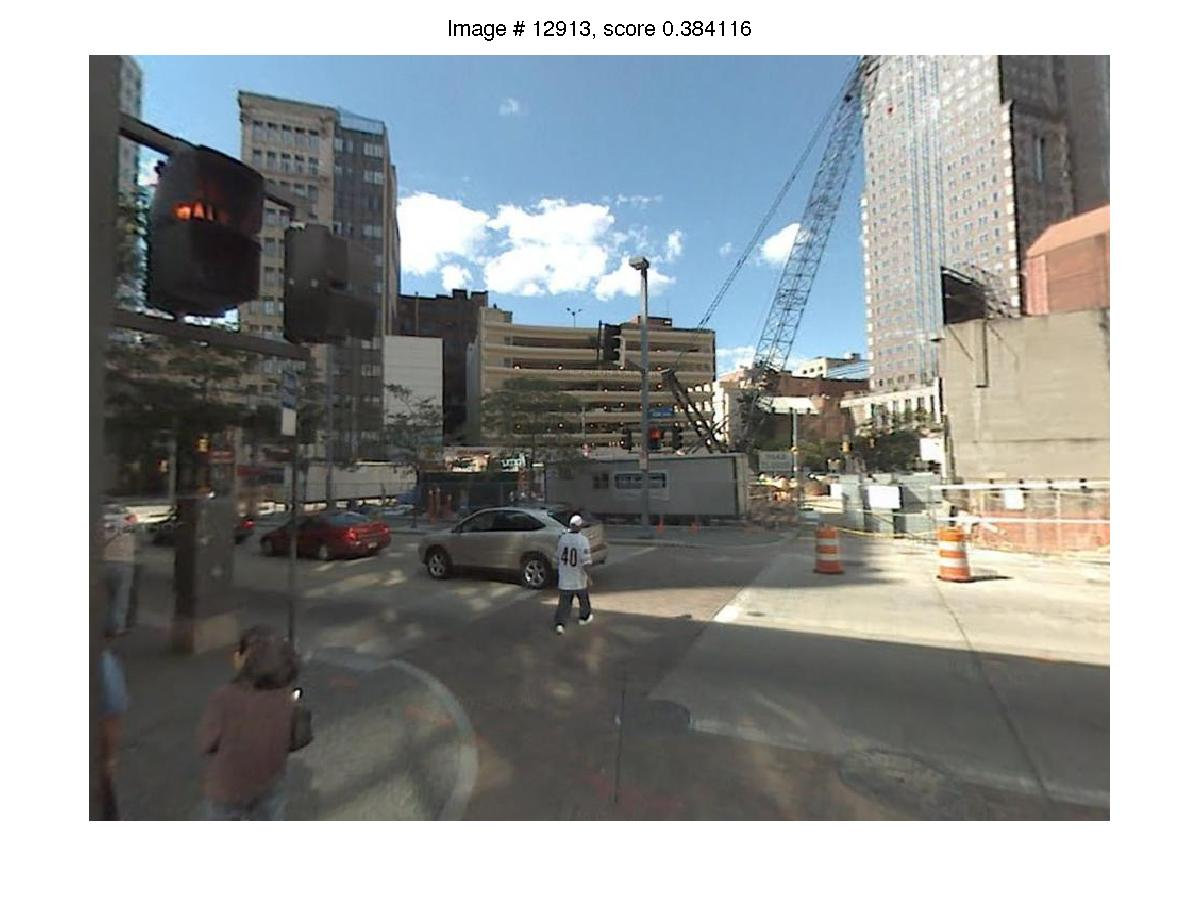
\includegraphics[trim = 55mm 40mm 55mm 30mm, clip=true,width=0.30\linewidth]{sup1693/raw03.jpg}}
		\colorbox{myCopper4}{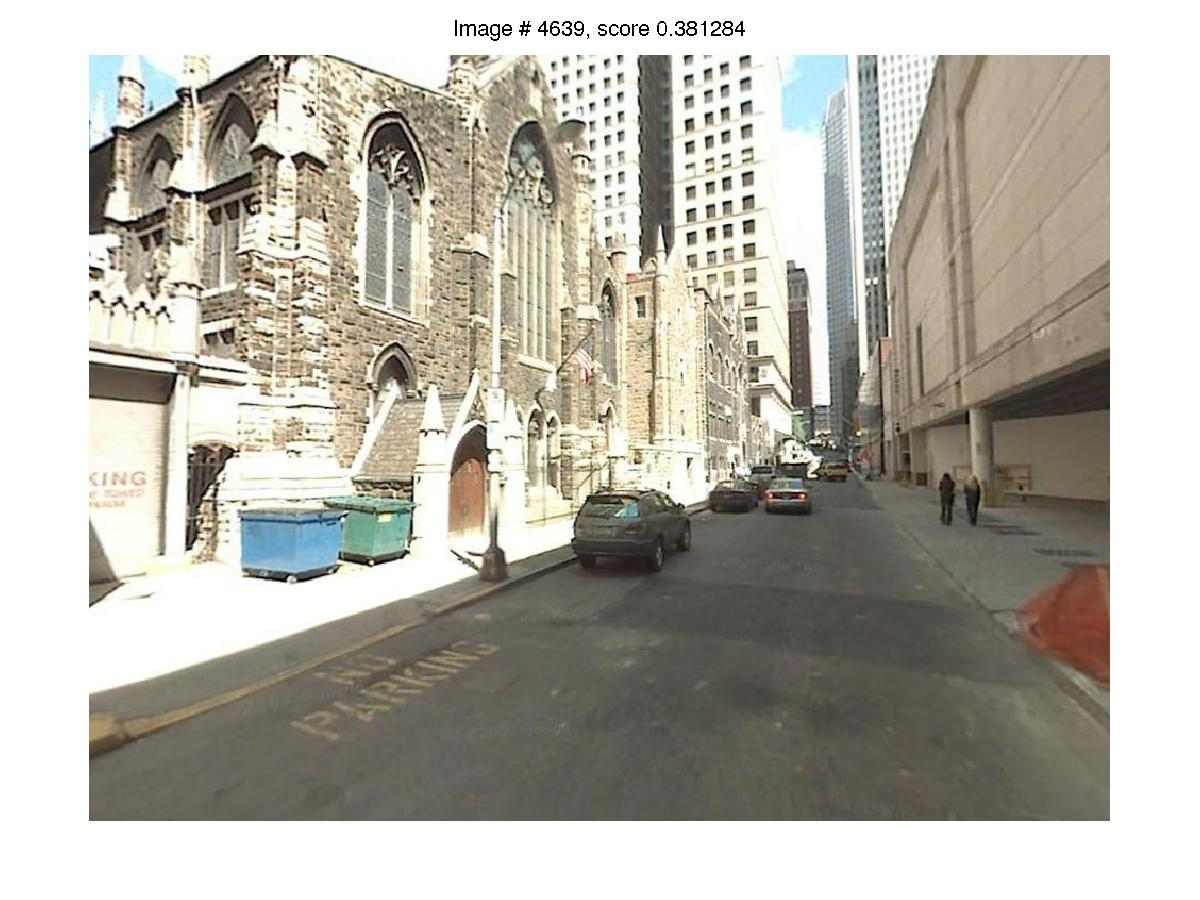
\includegraphics[trim = 55mm 40mm 55mm 30mm, clip=true,width=0.30\linewidth]{sup1693/raw04.jpg}}
		\colorbox{myCopper5}{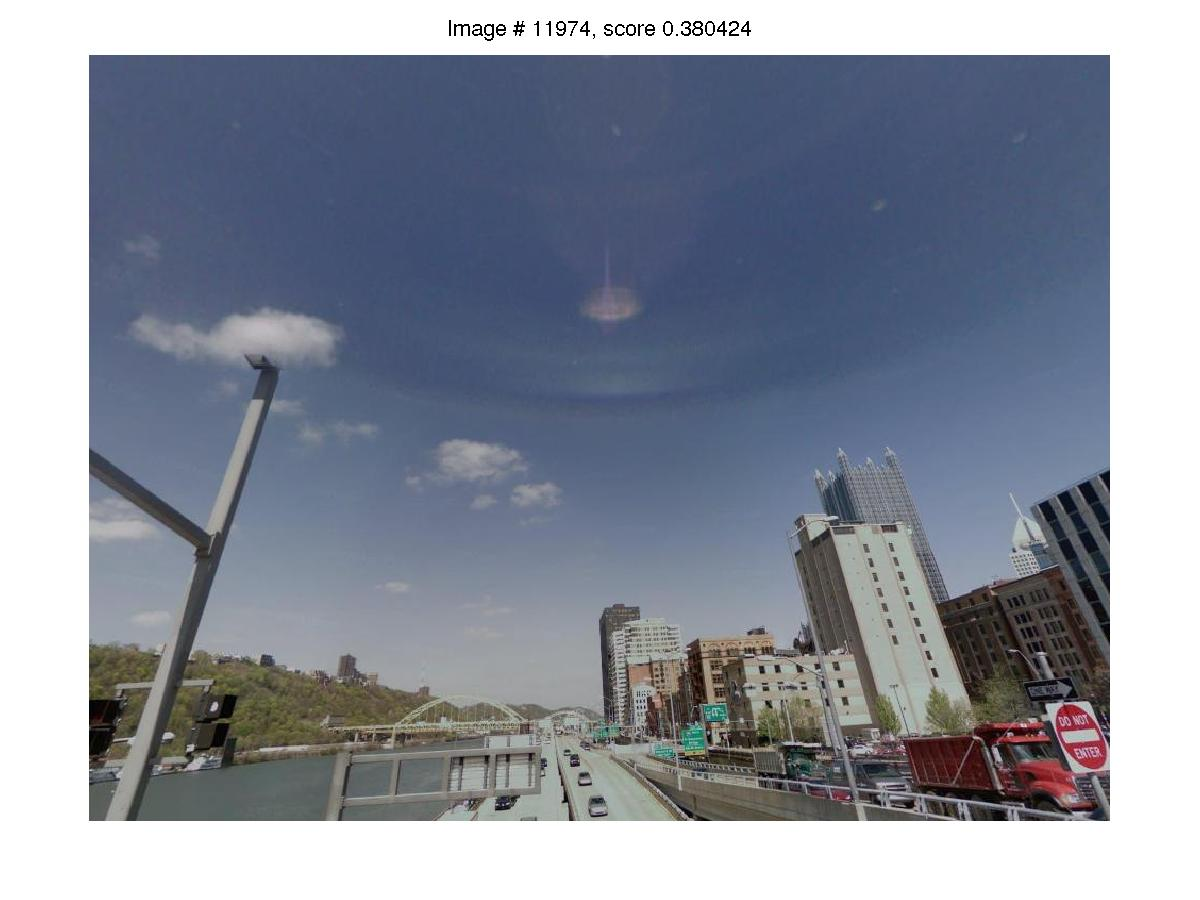
\includegraphics[trim = 55mm 40mm 55mm 30mm, clip=true,width=0.30\linewidth]{sup1693/raw05.jpg}} \\
		\textcolor{myWhite}{xxxxxx}3. \hspace{0.25\linewidth}4. \hspace{0.25\linewidth}5. \\
	\end{minipage} 
	\begin{minipage}{0.45\linewidth}
		\colorbox{myGrey}{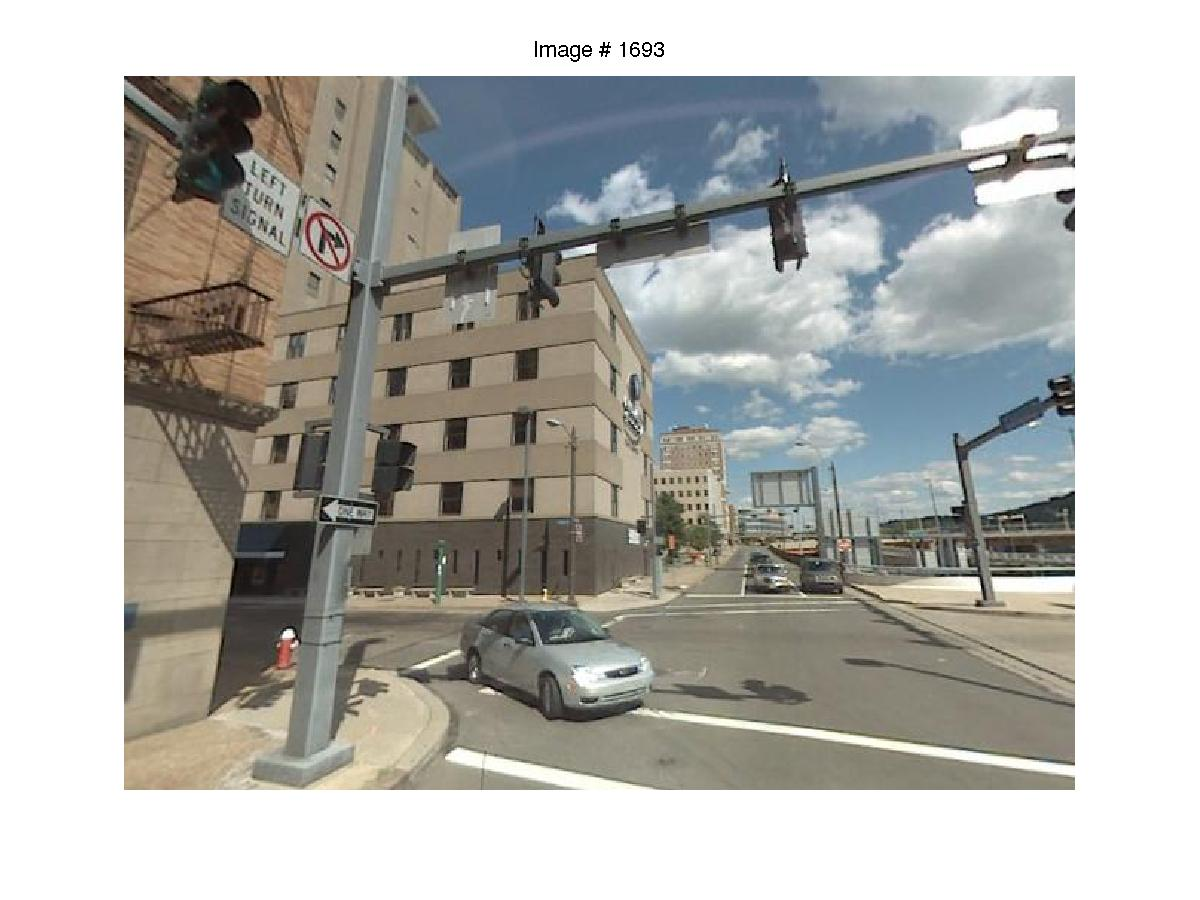
\includegraphics[trim = 55mm 40mm 55mm 30mm, clip=true,width=0.30\linewidth]{sup1693/query.jpg}}
		\colorbox{myCopper1}{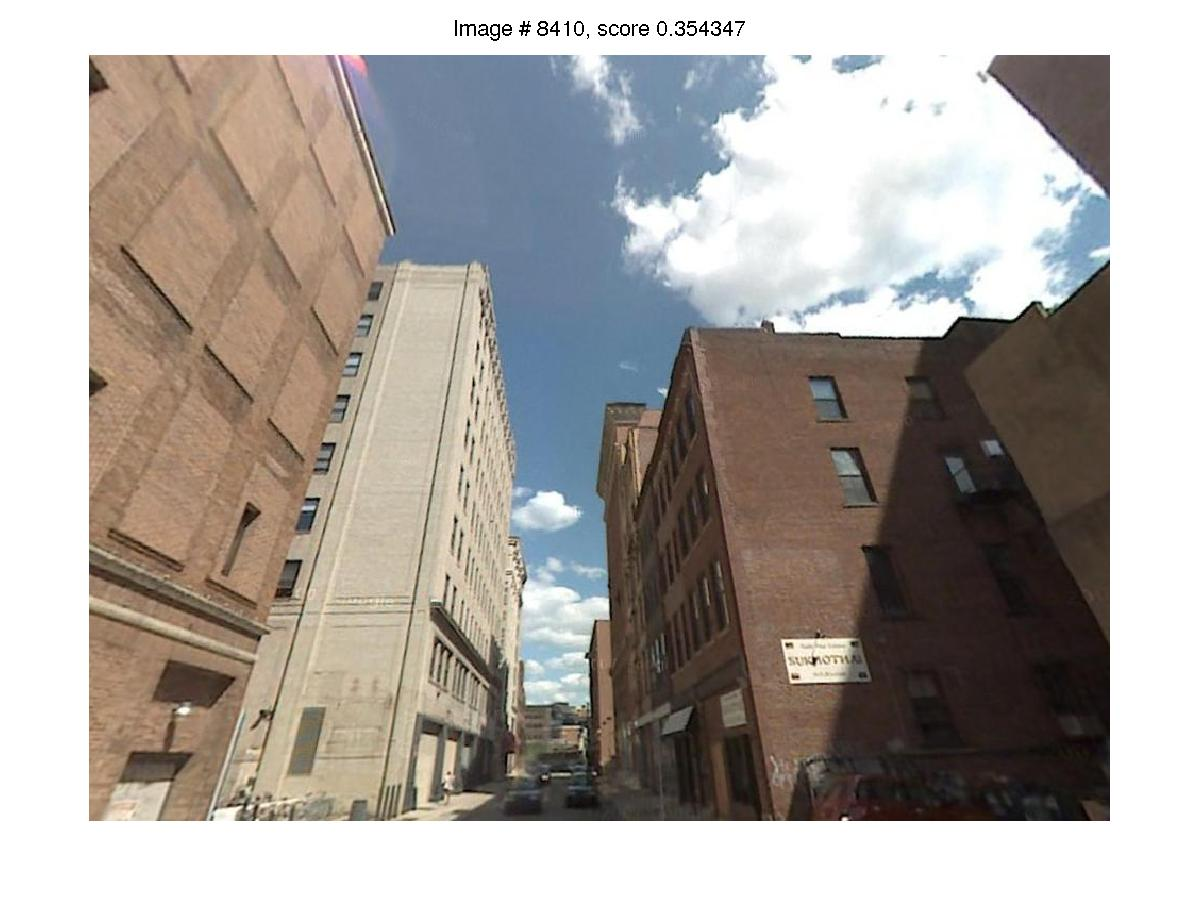
\includegraphics[trim = 55mm 40mm 55mm 30mm, clip=true,width=0.30\linewidth]{sup1693/svm01.jpg}}
		\colorbox{myCopper2}{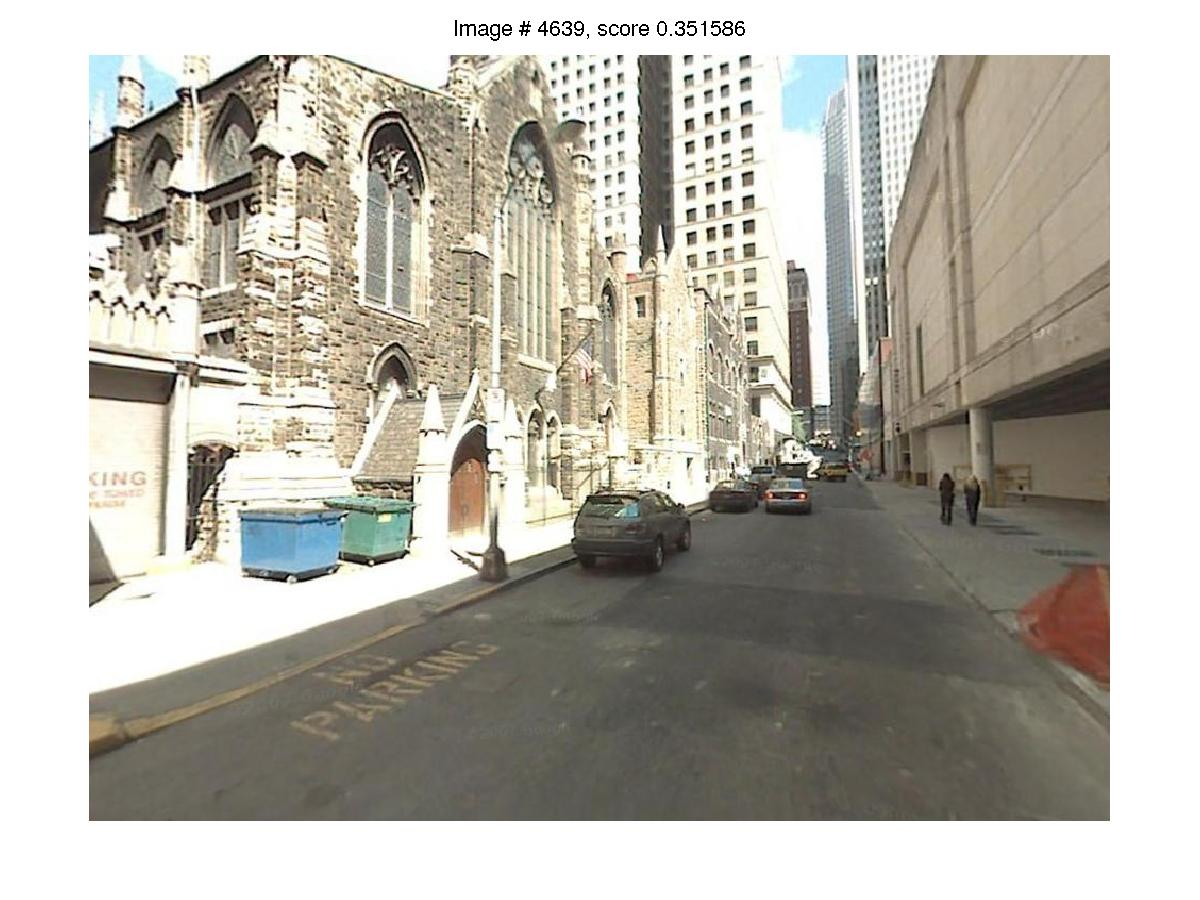
\includegraphics[trim = 55mm 40mm 55mm 30mm, clip=true,width=0.30\linewidth]{sup1693/svm02.jpg}}	\\
		\textcolor{myWhite}{xxxxxx}Query \hspace{0.25\linewidth}1. \hspace{0.25\linewidth}2. \\
		\colorbox{myGreen}{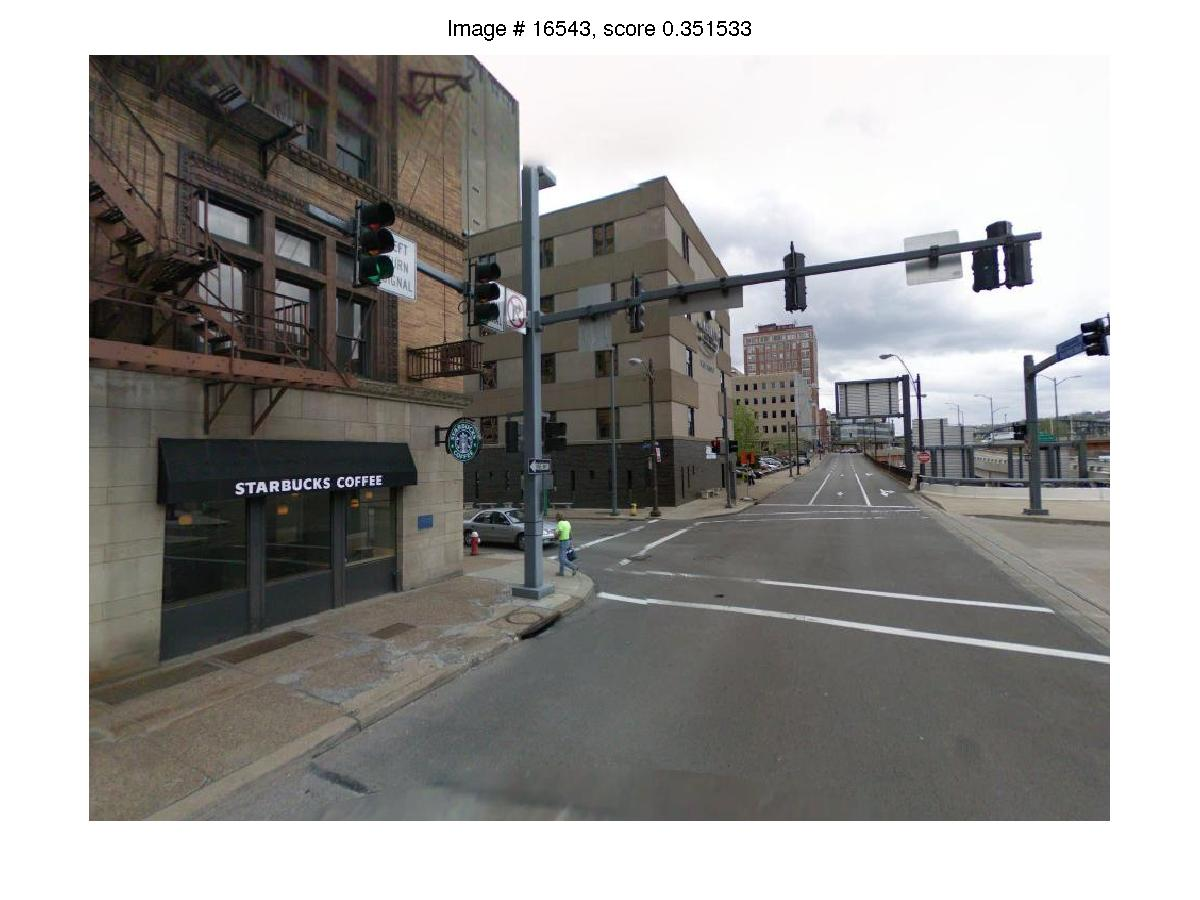
\includegraphics[trim = 55mm 40mm 55mm 30mm, clip=true,width=0.30\linewidth]{sup1693/svm03.jpg}}
		\colorbox{myCopper4}{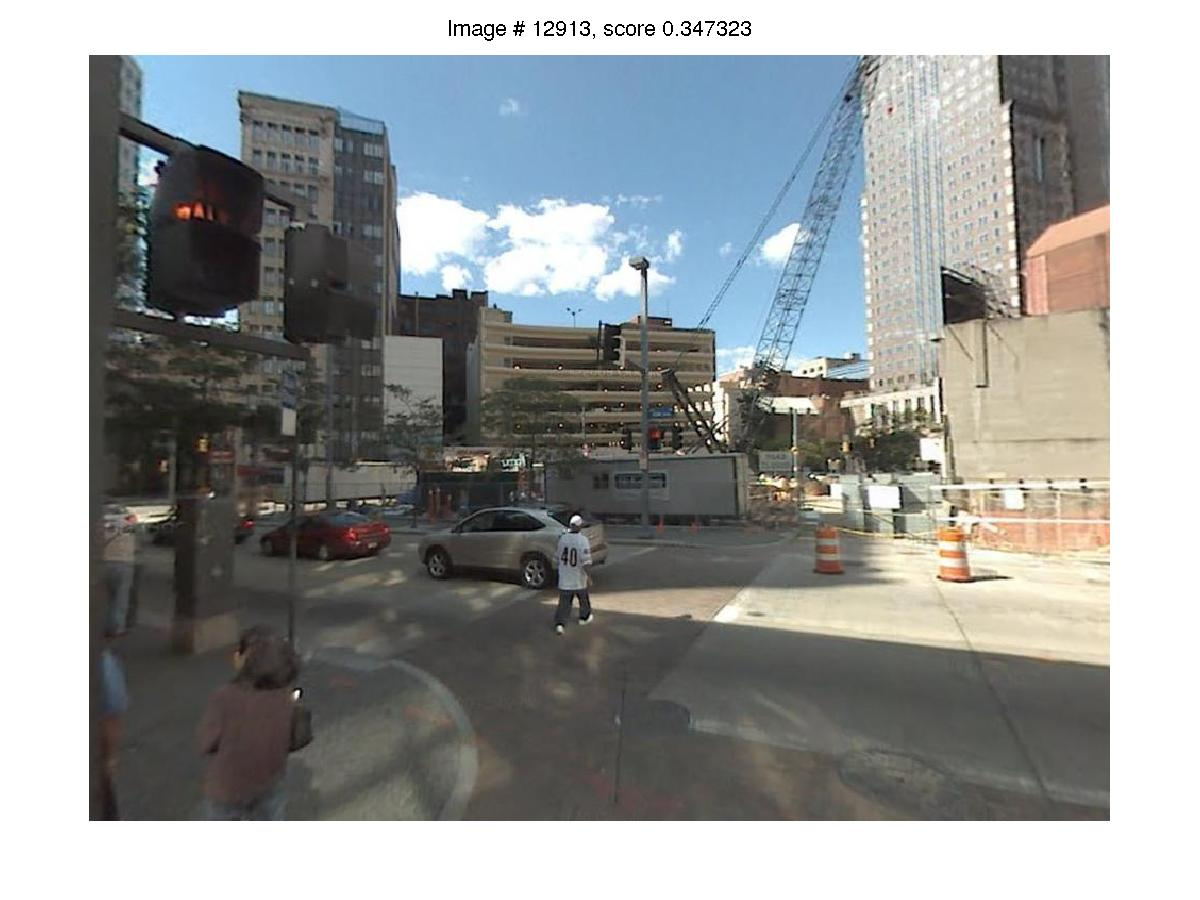
\includegraphics[trim = 55mm 40mm 55mm 30mm, clip=true,width=0.30\linewidth]{sup1693/svm04.jpg}}
		\colorbox{myCopper5}{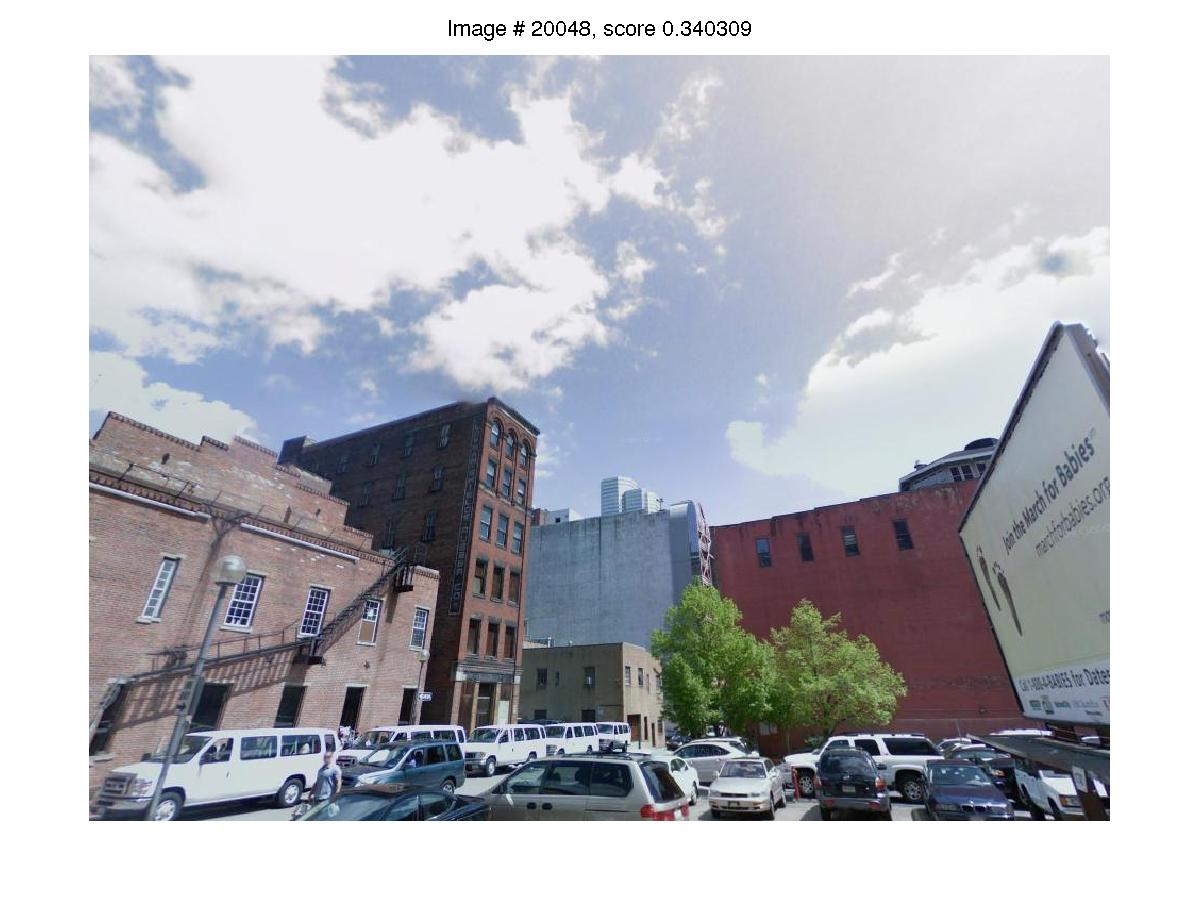
\includegraphics[trim = 55mm 40mm 55mm 30mm, clip=true,width=0.30\linewidth]{sup1693/svm05.jpg}}  \\
		\textcolor{myWhite}{xxxxxx}3. \hspace{0.25\linewidth}4. \hspace{0.25\linewidth}5. \\
	\end{minipage}
	%%\caption{Example sup1693} 
\end{figure}


\begin{figure}
	\begin{minipage}{0.45\linewidth}
		\center
		(raw FV128 baseline) \\
		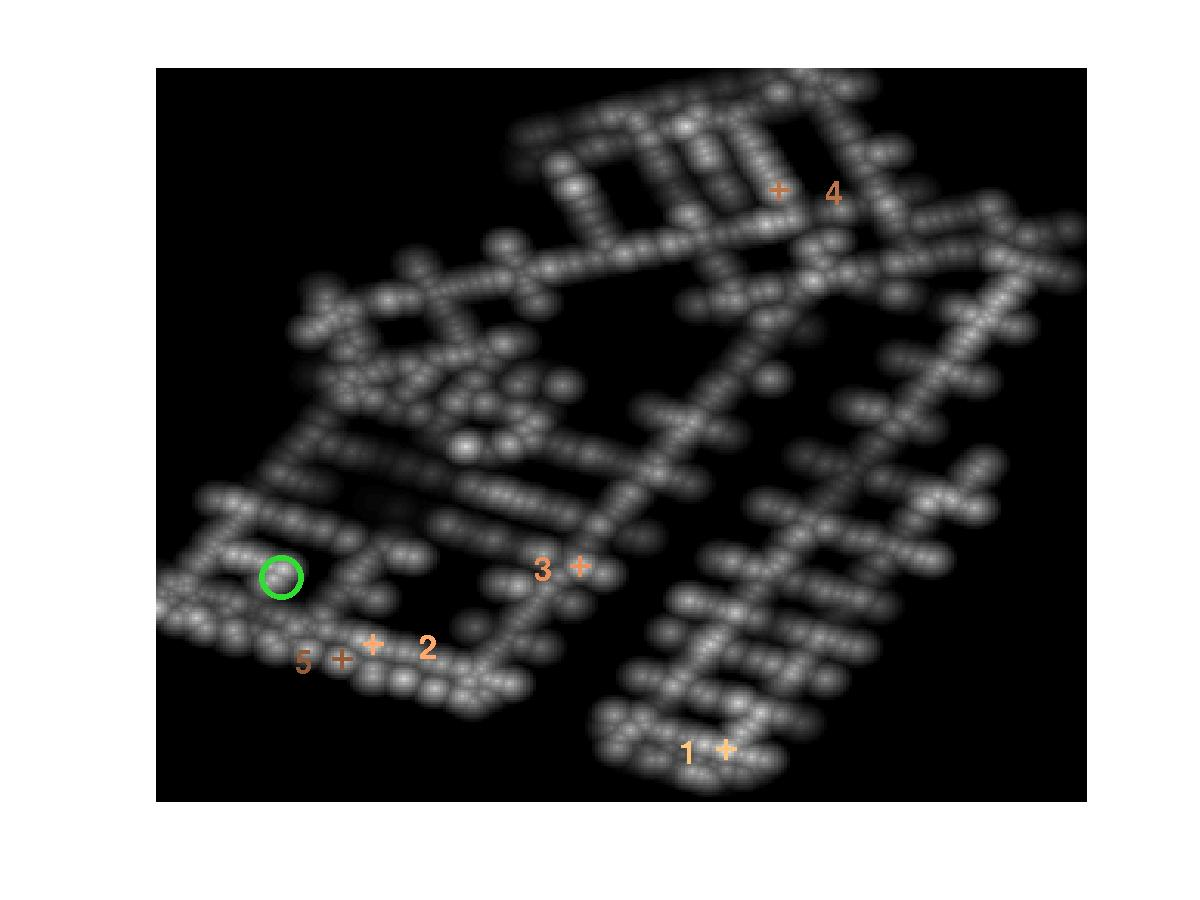
\includegraphics[trim = 55mm 40mm 55mm 25mm, clip=true,width=\linewidth]{sup1812/heatRaw.jpg}
	\end{minipage} 
	\begin{minipage}{0.45\linewidth}
		\center
		(e-SVM FV128) \\
		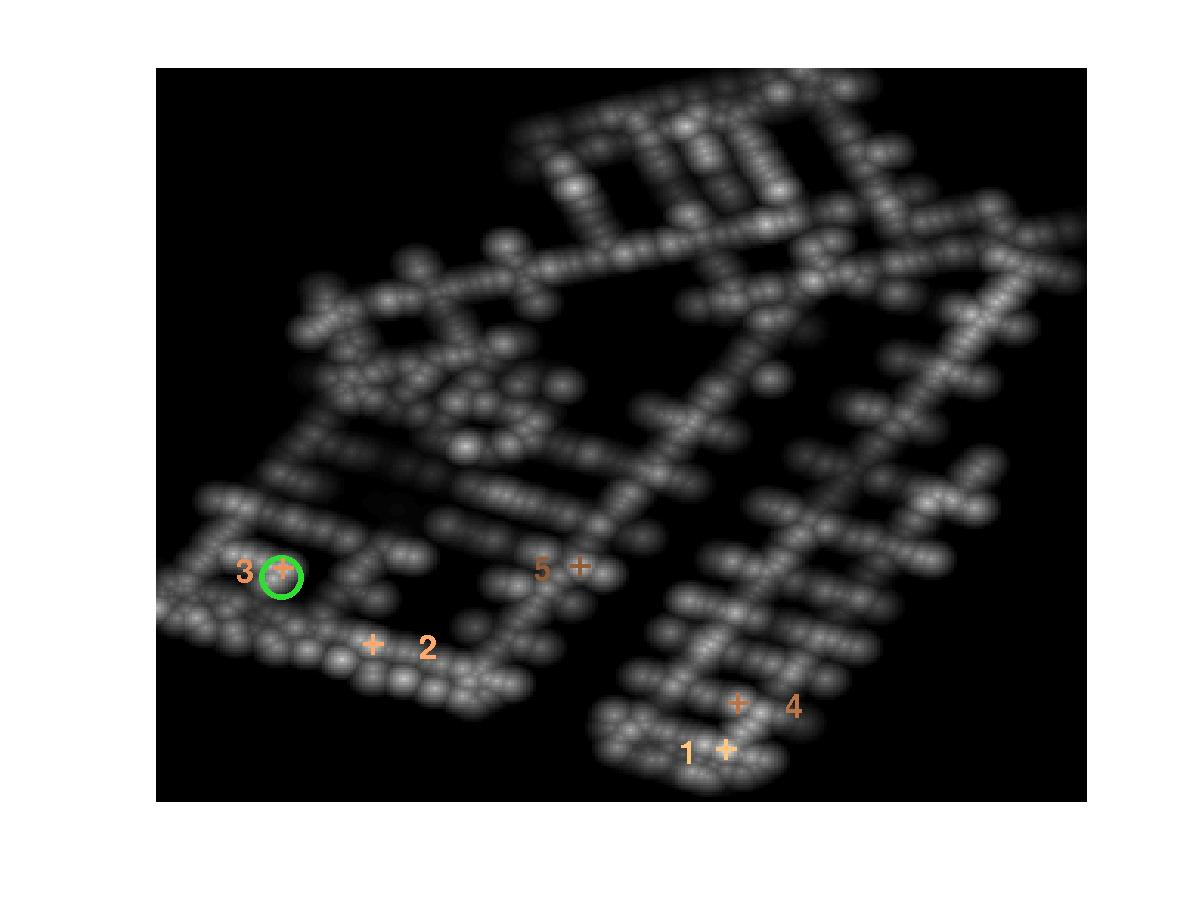
\includegraphics[trim = 55mm 40mm 55mm 25mm, clip=true,width=\linewidth]{sup1812/heatSvm.jpg}
	\end{minipage} 
	\\
	\textcolor{myWhite}{xxx}\\
	\begin{minipage}{0.45\linewidth}
		\colorbox{myGrey}{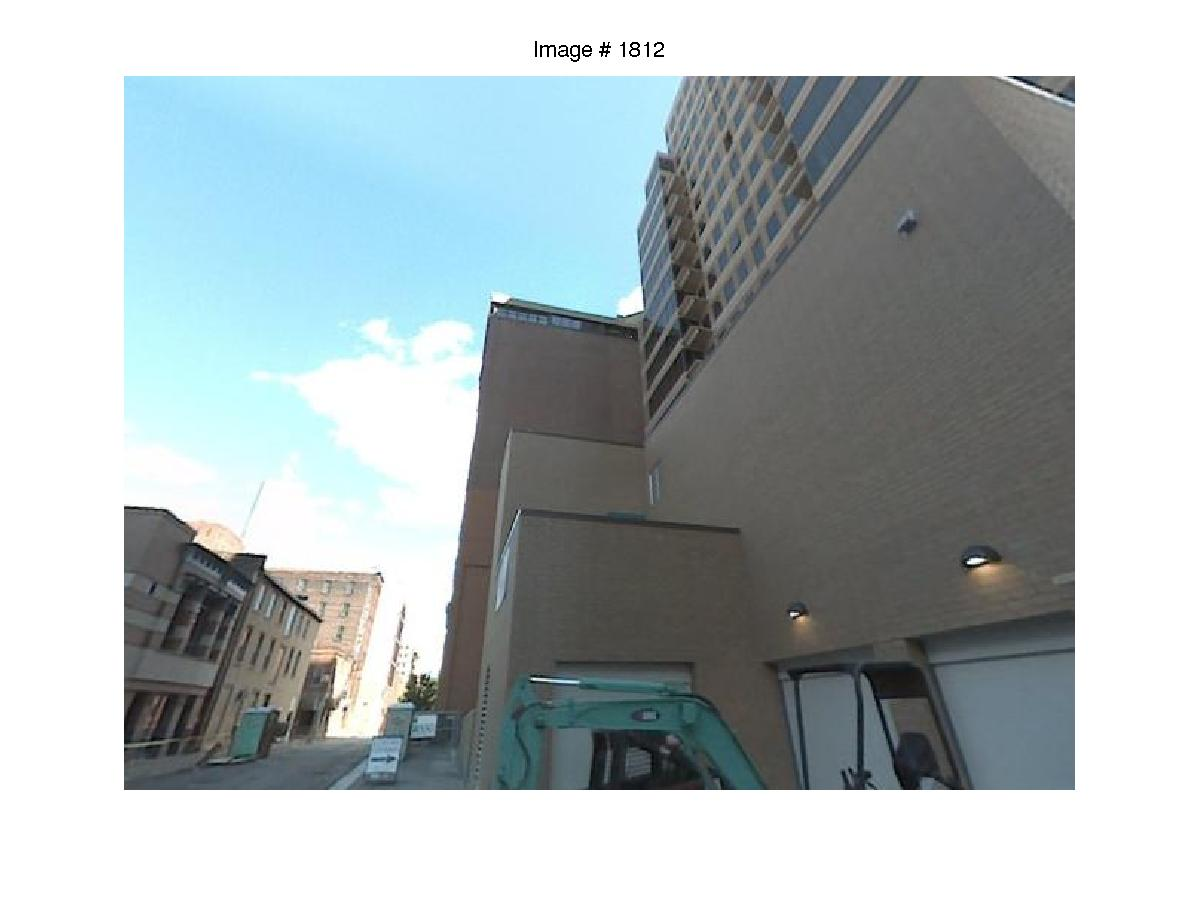
\includegraphics[trim = 55mm 40mm 55mm 30mm, clip=true,width=0.30\linewidth]{sup1812/query.jpg}}
		\colorbox{myCopper1}{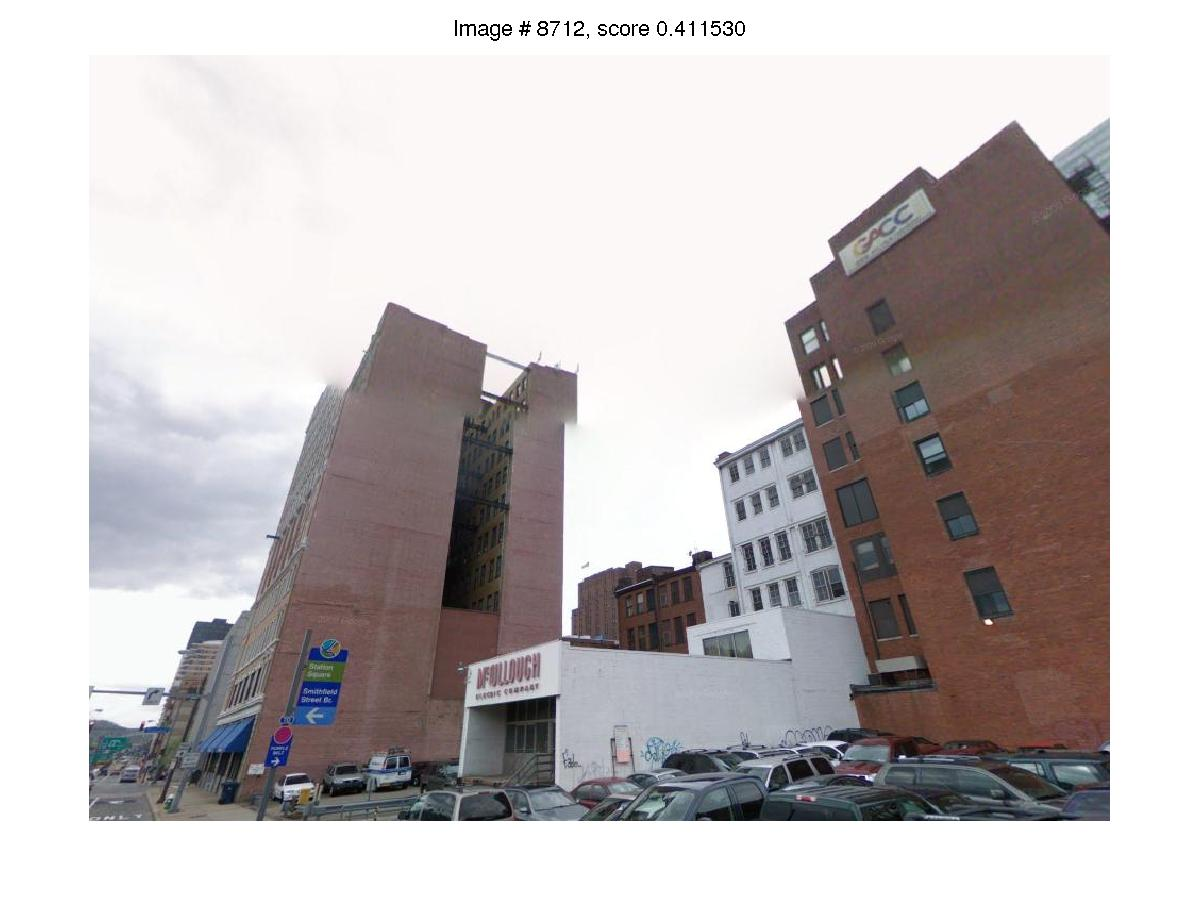
\includegraphics[trim = 55mm 40mm 55mm 30mm, clip=true,width=0.30\linewidth]{sup1812/raw01.jpg}}
		\colorbox{myCopper2}{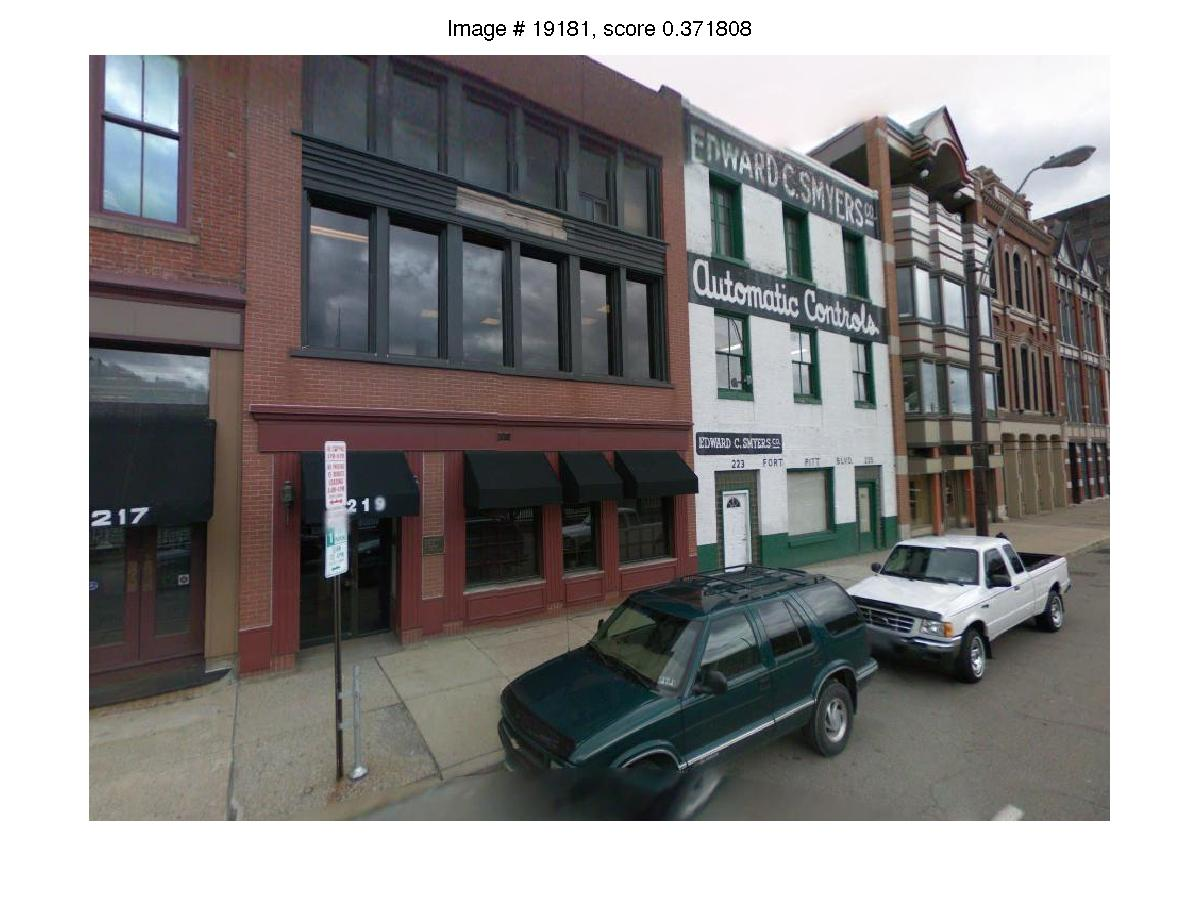
\includegraphics[trim = 55mm 40mm 55mm 30mm, clip=true,width=0.30\linewidth]{sup1812/raw02.jpg}}	\\
		\textcolor{myWhite}{xxxxxx}Query \hspace{0.25\linewidth}1. \hspace{0.25\linewidth}2. \\
		\colorbox{myCopper3}{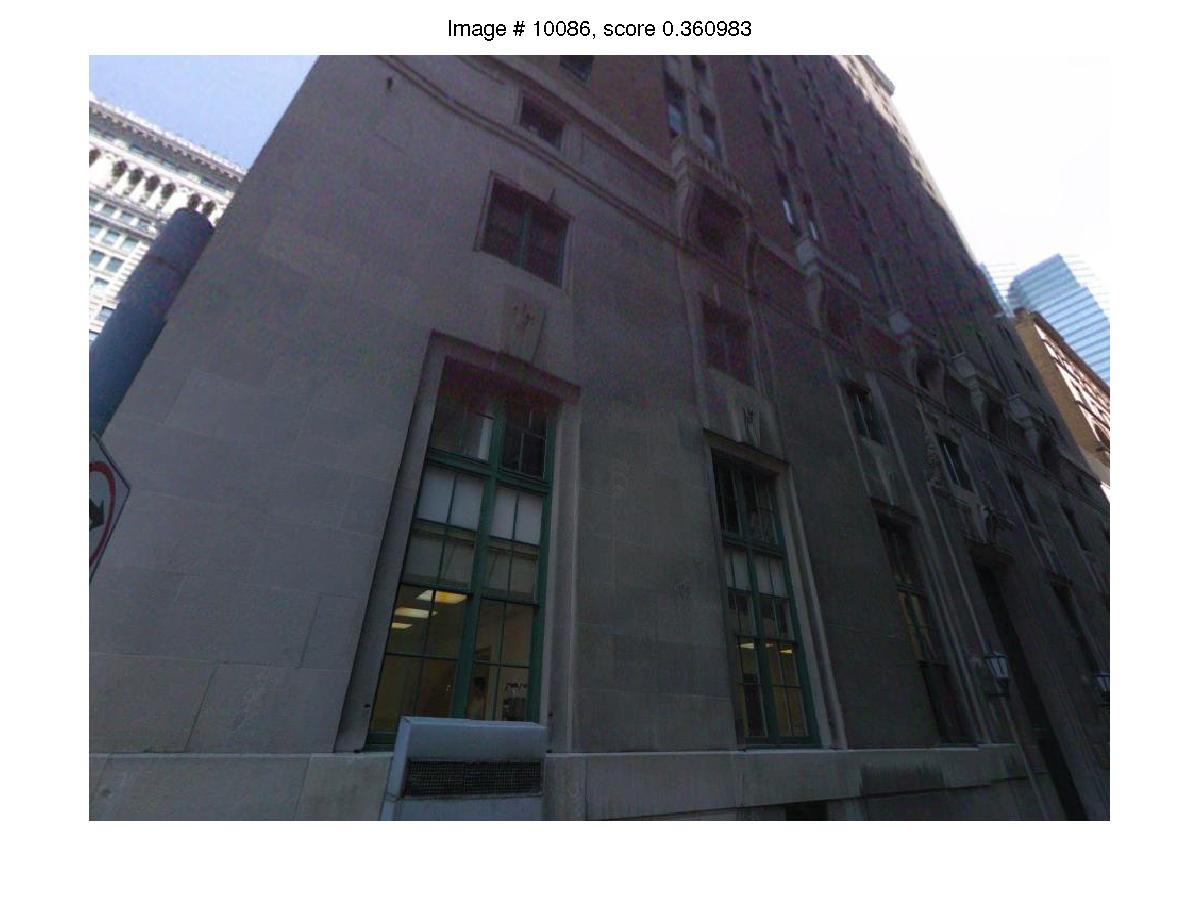
\includegraphics[trim = 55mm 40mm 55mm 30mm, clip=true,width=0.30\linewidth]{sup1812/raw03.jpg}}
		\colorbox{myCopper4}{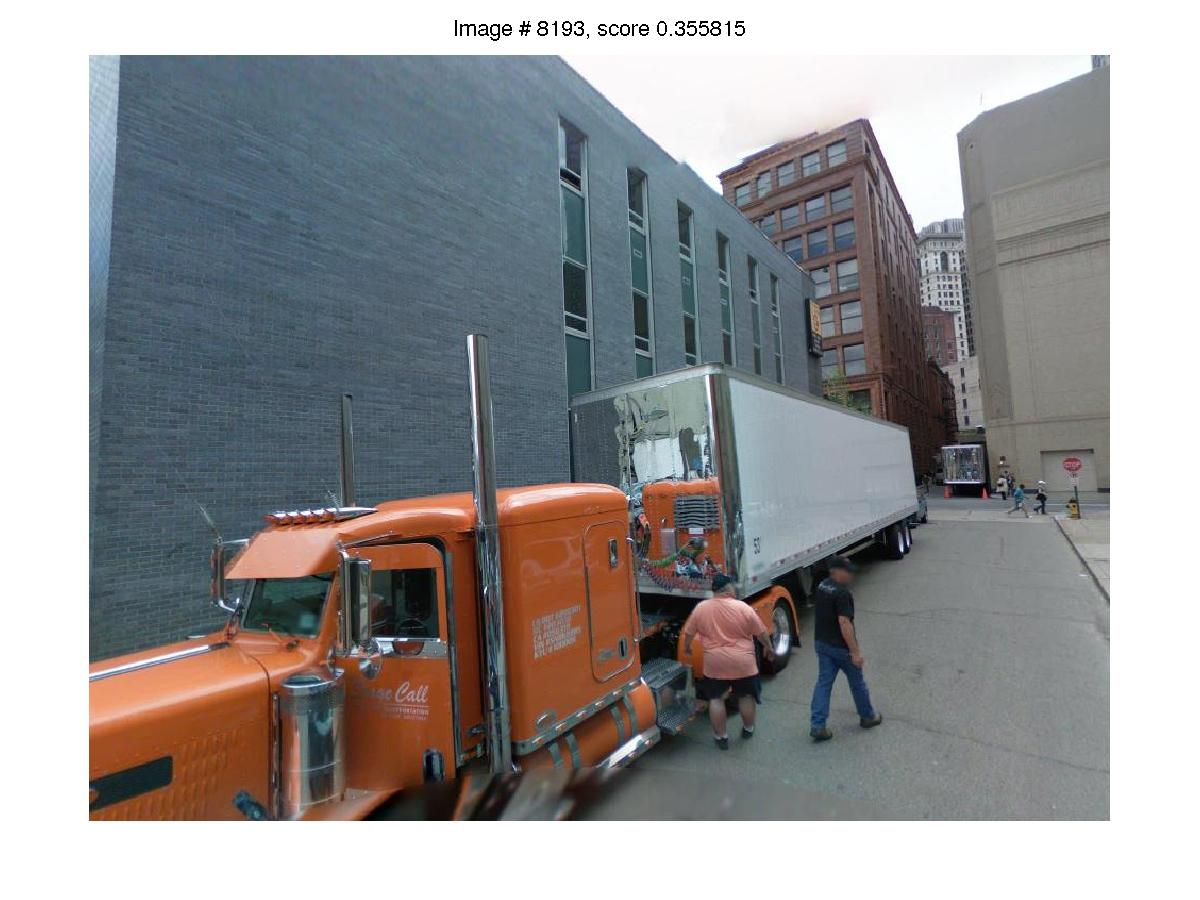
\includegraphics[trim = 55mm 40mm 55mm 30mm, clip=true,width=0.30\linewidth]{sup1812/raw04.jpg}}
		\colorbox{myCopper5}{\includegraphics[trim = 55mm 40mm 55mm 30mm, clip=true,width=0.30\linewidth]{sup1812/raw05.jpg}} \\
		\textcolor{myWhite}{xxxxxx}3. \hspace{0.25\linewidth}4. \hspace{0.25\linewidth}5. \\
	\end{minipage} 
	\begin{minipage}{0.45\linewidth}
		\colorbox{myGrey}{\includegraphics[trim = 55mm 40mm 55mm 30mm, clip=true,width=0.30\linewidth]{sup1812/query.jpg}}
		\colorbox{myCopper1}{\includegraphics[trim = 55mm 40mm 55mm 30mm, clip=true,width=0.30\linewidth]{sup1812/svm01.jpg}}
		\colorbox{myCopper2}{\includegraphics[trim = 55mm 40mm 55mm 30mm, clip=true,width=0.30\linewidth]{sup1812/svm02.jpg}}	\\
		\textcolor{myWhite}{xxxxxx}Query \hspace{0.25\linewidth}1. \hspace{0.25\linewidth}2. \\
		\colorbox{myGreen}{\includegraphics[trim = 55mm 40mm 55mm 30mm, clip=true,width=0.30\linewidth]{sup1812/svm03.jpg}}
		\colorbox{myCopper4}{\includegraphics[trim = 55mm 40mm 55mm 30mm, clip=true,width=0.30\linewidth]{sup1812/svm04.jpg}}
		\colorbox{myCopper5}{\includegraphics[trim = 55mm 40mm 55mm 30mm, clip=true,width=0.30\linewidth]{sup1812/svm05.jpg}}  \\
		\textcolor{myWhite}{xxxxxx}3. \hspace{0.25\linewidth}4. \hspace{0.25\linewidth}5. \\
	\end{minipage}
	%%\caption{Example sup1812} 
\end{figure}

\begin{figure}
	\begin{minipage}{0.45\linewidth}
		\center
		(raw FV128 baseline) \\
		\includegraphics[trim = 55mm 40mm 55mm 25mm, clip=true,width=\linewidth]{sup1957/heatRaw.jpg}
	\end{minipage} 
	\begin{minipage}{0.45\linewidth}
		\center
		(e-SVM FV128) \\
		\includegraphics[trim = 55mm 40mm 55mm 25mm, clip=true,width=\linewidth]{sup1957/heatSvm.jpg}
	\end{minipage} 
	\\
	\textcolor{myWhite}{xxx}\\
	\begin{minipage}{0.45\linewidth}
		\colorbox{myGrey}{\includegraphics[trim = 55mm 40mm 55mm 30mm, clip=true,width=0.30\linewidth]{sup1957/query.jpg}}
		\colorbox{myCopper1}{\includegraphics[trim = 55mm 40mm 55mm 30mm, clip=true,width=0.30\linewidth]{sup1957/raw01.jpg}}
		\colorbox{myCopper2}{\includegraphics[trim = 55mm 40mm 55mm 30mm, clip=true,width=0.30\linewidth]{sup1957/raw02.jpg}}	\\
		\textcolor{myWhite}{xxxxxx}Query \hspace{0.25\linewidth}1. \hspace{0.25\linewidth}2. \\
		\colorbox{myCopper3}{\includegraphics[trim = 55mm 40mm 55mm 30mm, clip=true,width=0.30\linewidth]{sup1957/raw03.jpg}}
		\colorbox{myCopper4}{\includegraphics[trim = 55mm 40mm 55mm 30mm, clip=true,width=0.30\linewidth]{sup1957/raw04.jpg}}
		\colorbox{myCopper5}{\includegraphics[trim = 55mm 40mm 55mm 30mm, clip=true,width=0.30\linewidth]{sup1957/raw05.jpg}} \\
		\textcolor{myWhite}{xxxxxx}3. \hspace{0.25\linewidth}4. \hspace{0.25\linewidth}5. \\
	\end{minipage} 
	\begin{minipage}{0.45\linewidth}
		\colorbox{myGrey}{\includegraphics[trim = 55mm 40mm 55mm 30mm, clip=true,width=0.30\linewidth]{sup1957/query.jpg}}
		\colorbox{myCopper1}{\includegraphics[trim = 55mm 40mm 55mm 30mm, clip=true,width=0.30\linewidth]{sup1957/svm01.jpg}}
		\colorbox{myCopper2}{\includegraphics[trim = 55mm 40mm 55mm 30mm, clip=true,width=0.30\linewidth]{sup1957/svm02.jpg}}	\\
		\textcolor{myWhite}{xxxxxx}Query \hspace{0.25\linewidth}1. \hspace{0.25\linewidth}2. \\
		\colorbox{myGreen}{\includegraphics[trim = 55mm 40mm 55mm 30mm, clip=true,width=0.30\linewidth]{sup1957/svm03.jpg}}
		\colorbox{myCopper4}{\includegraphics[trim = 55mm 40mm 55mm 30mm, clip=true,width=0.30\linewidth]{sup1957/svm04.jpg}}
		\colorbox{myCopper5}{\includegraphics[trim = 55mm 40mm 55mm 30mm, clip=true,width=0.30\linewidth]{sup1957/svm05.jpg}}  \\
		\textcolor{myWhite}{xxxxxx}3. \hspace{0.25\linewidth}4. \hspace{0.25\linewidth}5. \\
	\end{minipage}
	%%\caption{Example sup1957} 
\end{figure}



\begin{figure}
	\begin{minipage}{0.45\linewidth}
		\center
		(raw FV128 baseline) \\
		\includegraphics[trim = 55mm 40mm 55mm 25mm, clip=true,width=\linewidth]{sup1962/heatRaw.jpg}
	\end{minipage} 
	\begin{minipage}{0.45\linewidth}
		\center
		(e-SVM FV128) \\
		\includegraphics[trim = 55mm 40mm 55mm 25mm, clip=true,width=\linewidth]{sup1962/heatSvm.jpg}
	\end{minipage} 
	\\
	\textcolor{myWhite}{xxx}\\
	\begin{minipage}{0.45\linewidth}
		\colorbox{myGrey}{\includegraphics[trim = 55mm 40mm 55mm 30mm, clip=true,width=0.30\linewidth]{sup1962/query.jpg}}
		\colorbox{myCopper1}{\includegraphics[trim = 55mm 40mm 55mm 30mm, clip=true,width=0.30\linewidth]{sup1962/raw01.jpg}}
		\colorbox{myCopper2}{\includegraphics[trim = 55mm 40mm 55mm 30mm, clip=true,width=0.30\linewidth]{sup1962/raw02.jpg}}	\\
		\textcolor{myWhite}{xxxxxx}Query \hspace{0.25\linewidth}1. \hspace{0.25\linewidth}2. \\
		\colorbox{myCopper3}{\includegraphics[trim = 55mm 40mm 55mm 30mm, clip=true,width=0.30\linewidth]{sup1962/raw03.jpg}}
		\colorbox{myCopper4}{\includegraphics[trim = 55mm 40mm 55mm 30mm, clip=true,width=0.30\linewidth]{sup1962/raw04.jpg}}
		\colorbox{myCopper5}{\includegraphics[trim = 55mm 40mm 55mm 30mm, clip=true,width=0.30\linewidth]{sup1962/raw05.jpg}} \\
		\textcolor{myWhite}{xxxxxx}3. \hspace{0.25\linewidth}4. \hspace{0.25\linewidth}5. \\
	\end{minipage} 
	\begin{minipage}{0.45\linewidth}
		\colorbox{myGrey}{\includegraphics[trim = 55mm 40mm 55mm 30mm, clip=true,width=0.30\linewidth]{sup1962/query.jpg}}
		\colorbox{myCopper1}{\includegraphics[trim = 55mm 40mm 55mm 30mm, clip=true,width=0.30\linewidth]{sup1962/svm01.jpg}}
		\colorbox{myGreen}{\includegraphics[trim = 55mm 40mm 55mm 30mm, clip=true,width=0.30\linewidth]{sup1962/svm02.jpg}}	\\
		\textcolor{myWhite}{xxxxxx}Query \hspace{0.25\linewidth}1. \hspace{0.25\linewidth}2. \\
		\colorbox{myCopper3}{\includegraphics[trim = 55mm 40mm 55mm 30mm, clip=true,width=0.30\linewidth]{sup1962/svm03.jpg}}
		\colorbox{myCopper4}{\includegraphics[trim = 55mm 40mm 55mm 30mm, clip=true,width=0.30\linewidth]{sup1962/svm04.jpg}}
		\colorbox{myCopper5}{\includegraphics[trim = 55mm 40mm 55mm 30mm, clip=true,width=0.30\linewidth]{sup1962/svm05.jpg}}  \\
		\textcolor{myWhite}{xxxxxx}3. \hspace{0.25\linewidth}4. \hspace{0.25\linewidth}5. \\
	\end{minipage}
	%%\caption{Example sup1962} 
\end{figure}




\begin{figure}
	\begin{minipage}{0.45\linewidth}
		\center
		(raw FV128 baseline) \\
		\includegraphics[trim = 55mm 40mm 55mm 25mm, clip=true,width=\linewidth]{sup2358/heatRaw.jpg}
	\end{minipage} 
	\begin{minipage}{0.45\linewidth}
		\center
		(e-SVM FV128) \\
		\includegraphics[trim = 55mm 40mm 55mm 25mm, clip=true,width=\linewidth]{sup2358/heatSvm.jpg}
	\end{minipage} 
	\\
	\textcolor{myWhite}{xxx}\\
	\begin{minipage}{0.45\linewidth}
		\colorbox{myGrey}{\includegraphics[trim = 55mm 40mm 55mm 30mm, clip=true,width=0.30\linewidth]{sup2358/query.jpg}}
		\colorbox{myCopper1}{\includegraphics[trim = 55mm 40mm 55mm 30mm, clip=true,width=0.30\linewidth]{sup2358/raw01.jpg}}
		\colorbox{myCopper2}{\includegraphics[trim = 55mm 40mm 55mm 30mm, clip=true,width=0.30\linewidth]{sup2358/raw02.jpg}}	\\
		\textcolor{myWhite}{xxxxxx}Query \hspace{0.25\linewidth}1. \hspace{0.25\linewidth}2. \\
		\colorbox{myCopper3}{\includegraphics[trim = 55mm 40mm 55mm 30mm, clip=true,width=0.30\linewidth]{sup2358/raw03.jpg}}
		\colorbox{myCopper4}{\includegraphics[trim = 55mm 40mm 55mm 30mm, clip=true,width=0.30\linewidth]{sup2358/raw04.jpg}}
		\colorbox{myCopper5}{\includegraphics[trim = 55mm 40mm 55mm 30mm, clip=true,width=0.30\linewidth]{sup2358/raw05.jpg}} \\
		\textcolor{myWhite}{xxxxxx}3. \hspace{0.25\linewidth}4. \hspace{0.25\linewidth}5. \\
	\end{minipage} 
	\begin{minipage}{0.45\linewidth}
		\colorbox{myGrey}{\includegraphics[trim = 55mm 40mm 55mm 30mm, clip=true,width=0.30\linewidth]{sup2358/query.jpg}}
		\colorbox{myCopper1}{\includegraphics[trim = 55mm 40mm 55mm 30mm, clip=true,width=0.30\linewidth]{sup2358/svm01.jpg}}
		\colorbox{myCopper2}{\includegraphics[trim = 55mm 40mm 55mm 30mm, clip=true,width=0.30\linewidth]{sup2358/svm02.jpg}}	\\
		\textcolor{myWhite}{xxxxxx}Query \hspace{0.25\linewidth}1. \hspace{0.25\linewidth}2. \\
		\colorbox{myCopper3}{\includegraphics[trim = 55mm 40mm 55mm 30mm, clip=true,width=0.30\linewidth]{sup2358/svm03.jpg}}
		\colorbox{myGreen}{\includegraphics[trim = 55mm 40mm 55mm 30mm, clip=true,width=0.30\linewidth]{sup2358/svm04.jpg}}
		\colorbox{myCopper5}{\includegraphics[trim = 55mm 40mm 55mm 30mm, clip=true,width=0.30\linewidth]{sup2358/svm05.jpg}}  \\
		\textcolor{myWhite}{xxxxxx}3. \hspace{0.25\linewidth}4. \hspace{0.25\linewidth}5. \\
	\end{minipage}
	%%\caption{Example sup2358} 
\end{figure}


\begin{figure}
	\begin{minipage}{0.45\linewidth}
		\center
		(raw FV128 baseline) \\
		\includegraphics[trim = 55mm 40mm 55mm 25mm, clip=true,width=\linewidth]{sup2569/heatRaw.jpg}
	\end{minipage} 
	\begin{minipage}{0.45\linewidth}
		\center
		(e-SVM FV128) \\
		\includegraphics[trim = 55mm 40mm 55mm 25mm, clip=true,width=\linewidth]{sup2569/heatSvm.jpg}
	\end{minipage} 
	\\
	\textcolor{myWhite}{xxx}\\
	\begin{minipage}{0.45\linewidth}
		\colorbox{myGrey}{\includegraphics[trim = 55mm 40mm 55mm 30mm, clip=true,width=0.30\linewidth]{sup2569/query.jpg}}
		\colorbox{myCopper1}{\includegraphics[trim = 55mm 40mm 55mm 30mm, clip=true,width=0.30\linewidth]{sup2569/raw01.jpg}}
		\colorbox{myCopper2}{\includegraphics[trim = 55mm 40mm 55mm 30mm, clip=true,width=0.30\linewidth]{sup2569/raw02.jpg}}	\\
		\textcolor{myWhite}{xxxxxx}Query \hspace{0.25\linewidth}1. \hspace{0.25\linewidth}2. \\
		\colorbox{myCopper3}{\includegraphics[trim = 55mm 40mm 55mm 30mm, clip=true,width=0.30\linewidth]{sup2569/raw03.jpg}}
		\colorbox{myCopper4}{\includegraphics[trim = 55mm 40mm 55mm 30mm, clip=true,width=0.30\linewidth]{sup2569/raw04.jpg}}
		\colorbox{myCopper5}{\includegraphics[trim = 55mm 40mm 55mm 30mm, clip=true,width=0.30\linewidth]{sup2569/raw05.jpg}} \\
		\textcolor{myWhite}{xxxxxx}3. \hspace{0.25\linewidth}4. \hspace{0.25\linewidth}5. \\
	\end{minipage} 
	\begin{minipage}{0.45\linewidth}
		\colorbox{myGrey}{\includegraphics[trim = 55mm 40mm 55mm 30mm, clip=true,width=0.30\linewidth]{sup2569/query.jpg}}
		\colorbox{myCopper1}{\includegraphics[trim = 55mm 40mm 55mm 30mm, clip=true,width=0.30\linewidth]{sup2569/svm01.jpg}}
		\colorbox{myCopper2}{\includegraphics[trim = 55mm 40mm 55mm 30mm, clip=true,width=0.30\linewidth]{sup2569/svm02.jpg}}	\\
		\textcolor{myWhite}{xxxxxx}Query \hspace{0.25\linewidth}1. \hspace{0.25\linewidth}2. \\
		\colorbox{myCopper3}{\includegraphics[trim = 55mm 40mm 55mm 30mm, clip=true,width=0.30\linewidth]{sup2569/svm03.jpg}}
		\colorbox{myGreen}{\includegraphics[trim = 55mm 40mm 55mm 30mm, clip=true,width=0.30\linewidth]{sup2569/svm04.jpg}}
		\colorbox{myCopper5}{\includegraphics[trim = 55mm 40mm 55mm 30mm, clip=true,width=0.30\linewidth]{sup2569/svm05.jpg}}  \\
		\textcolor{myWhite}{xxxxxx}3. \hspace{0.25\linewidth}4. \hspace{0.25\linewidth}5. \\
	\end{minipage}
	%%\caption{Example sup2569} 
\end{figure}




\begin{figure}
	\begin{minipage}{0.45\linewidth}
		\center
		(raw FV128 baseline) \\
		\includegraphics[trim = 55mm 40mm 55mm 25mm, clip=true,width=\linewidth]{sup2602/heatRaw.jpg}
	\end{minipage} 
	\begin{minipage}{0.45\linewidth}
		\center
		(e-SVM FV128) \\
		\includegraphics[trim = 55mm 40mm 55mm 25mm, clip=true,width=\linewidth]{sup2602/heatSvm.jpg}
	\end{minipage} 
	\\
	\textcolor{myWhite}{xxx}\\
	\begin{minipage}{0.45\linewidth}
		\colorbox{myGrey}{\includegraphics[trim = 55mm 40mm 55mm 30mm, clip=true,width=0.30\linewidth]{sup2602/query.jpg}}
		\colorbox{myCopper1}{\includegraphics[trim = 55mm 40mm 55mm 30mm, clip=true,width=0.30\linewidth]{sup2602/raw01.jpg}}
		\colorbox{myCopper2}{\includegraphics[trim = 55mm 40mm 55mm 30mm, clip=true,width=0.30\linewidth]{sup2602/raw02.jpg}}	\\
		\textcolor{myWhite}{xxxxxx}Query \hspace{0.25\linewidth}1. \hspace{0.25\linewidth}2. \\
		\colorbox{myCopper3}{\includegraphics[trim = 55mm 40mm 55mm 30mm, clip=true,width=0.30\linewidth]{sup2602/raw03.jpg}}
		\colorbox{myCopper4}{\includegraphics[trim = 55mm 40mm 55mm 30mm, clip=true,width=0.30\linewidth]{sup2602/raw04.jpg}}
		\colorbox{myCopper5}{\includegraphics[trim = 55mm 40mm 55mm 30mm, clip=true,width=0.30\linewidth]{sup2602/raw05.jpg}} \\
		\textcolor{myWhite}{xxxxxx}3. \hspace{0.25\linewidth}4. \hspace{0.25\linewidth}5. \\
	\end{minipage} 
	\begin{minipage}{0.45\linewidth}
		\colorbox{myGrey}{\includegraphics[trim = 55mm 40mm 55mm 30mm, clip=true,width=0.30\linewidth]{sup2602/query.jpg}}
		\colorbox{myCopper1}{\includegraphics[trim = 55mm 40mm 55mm 30mm, clip=true,width=0.30\linewidth]{sup2602/svm01.jpg}}
		\colorbox{myCopper2}{\includegraphics[trim = 55mm 40mm 55mm 30mm, clip=true,width=0.30\linewidth]{sup2602/svm02.jpg}}	\\
		\textcolor{myWhite}{xxxxxx}Query \hspace{0.25\linewidth}1. \hspace{0.25\linewidth}2. \\
		\colorbox{myCopper3}{\includegraphics[trim = 55mm 40mm 55mm 30mm, clip=true,width=0.30\linewidth]{sup2602/svm03.jpg}}
		\colorbox{myGreen}{\includegraphics[trim = 55mm 40mm 55mm 30mm, clip=true,width=0.30\linewidth]{sup2602/svm04.jpg}}
		\colorbox{myCopper5}{\includegraphics[trim = 55mm 40mm 55mm 30mm, clip=true,width=0.30\linewidth]{sup2602/svm05.jpg}}  \\
		\textcolor{myWhite}{xxxxxx}3. \hspace{0.25\linewidth}4. \hspace{0.25\linewidth}5. \\
	\end{minipage}
	%%\caption{Example sup2602} 
\end{figure}




\begin{figure}
	\begin{minipage}{0.45\linewidth}
		\center
		(raw FV128 baseline) \\
		\includegraphics[trim = 55mm 40mm 55mm 25mm, clip=true,width=\linewidth]{sup2959/heatRaw.jpg}
	\end{minipage} 
	\begin{minipage}{0.45\linewidth}
		\center
		(e-SVM FV128) \\
		\includegraphics[trim = 55mm 40mm 55mm 25mm, clip=true,width=\linewidth]{sup2959/heatSvm.jpg}
	\end{minipage} 
	\\
	\textcolor{myWhite}{xxx}\\
	\begin{minipage}{0.45\linewidth}
		\colorbox{myGrey}{\includegraphics[trim = 55mm 40mm 55mm 30mm, clip=true,width=0.30\linewidth]{sup2959/query.jpg}}
		\colorbox{myCopper1}{\includegraphics[trim = 55mm 40mm 55mm 30mm, clip=true,width=0.30\linewidth]{sup2959/raw01.jpg}}
		\colorbox{myCopper2}{\includegraphics[trim = 55mm 40mm 55mm 30mm, clip=true,width=0.30\linewidth]{sup2959/raw02.jpg}}	\\
		\textcolor{myWhite}{xxxxxx}Query \hspace{0.25\linewidth}1. \hspace{0.25\linewidth}2. \\
		\colorbox{myCopper3}{\includegraphics[trim = 55mm 40mm 55mm 30mm, clip=true,width=0.30\linewidth]{sup2959/raw03.jpg}}
		\colorbox{myCopper4}{\includegraphics[trim = 55mm 40mm 55mm 30mm, clip=true,width=0.30\linewidth]{sup2959/raw04.jpg}}
		\colorbox{myCopper5}{\includegraphics[trim = 55mm 40mm 55mm 30mm, clip=true,width=0.30\linewidth]{sup2959/raw05.jpg}} \\
		\textcolor{myWhite}{xxxxxx}3. \hspace{0.25\linewidth}4. \hspace{0.25\linewidth}5. \\
	\end{minipage} 
	\begin{minipage}{0.45\linewidth}
		\colorbox{myGrey}{\includegraphics[trim = 55mm 40mm 55mm 30mm, clip=true,width=0.30\linewidth]{sup2959/query.jpg}}
		\colorbox{myCopper1}{\includegraphics[trim = 55mm 40mm 55mm 30mm, clip=true,width=0.30\linewidth]{sup2959/svm01.jpg}}
		\colorbox{myGreen}{\includegraphics[trim = 55mm 40mm 55mm 30mm, clip=true,width=0.30\linewidth]{sup2959/svm02.jpg}}	\\
		\textcolor{myWhite}{xxxxxx}Query \hspace{0.25\linewidth}1. \hspace{0.25\linewidth}2. \\
		\colorbox{myGreen}{\includegraphics[trim = 55mm 40mm 55mm 30mm, clip=true,width=0.30\linewidth]{sup2959/svm03.jpg}}
		\colorbox{myCopper4}{\includegraphics[trim = 55mm 40mm 55mm 30mm, clip=true,width=0.30\linewidth]{sup2959/svm04.jpg}}
		\colorbox{myCopper5}{\includegraphics[trim = 55mm 40mm 55mm 30mm, clip=true,width=0.30\linewidth]{sup2959/svm05.jpg}}  \\
		\textcolor{myWhite}{xxxxxx}3. \hspace{0.25\linewidth}4. \hspace{0.25\linewidth}5. \\
	\end{minipage}
	%%\caption{Example sup2959} 
\end{figure}



\begin{figure}
	\begin{minipage}{0.45\linewidth}
		\center
		(raw FV128 baseline) \\
		\includegraphics[trim = 55mm 40mm 55mm 25mm, clip=true,width=\linewidth]{sup2961/heatRaw.jpg}
	\end{minipage} 
	\begin{minipage}{0.45\linewidth}
		\center
		(e-SVM FV128) \\
		\includegraphics[trim = 55mm 40mm 55mm 25mm, clip=true,width=\linewidth]{sup2961/heatSvm.jpg}
	\end{minipage} 
	\\
	\textcolor{myWhite}{xxx}\\
	\begin{minipage}{0.45\linewidth}
		\colorbox{myGrey}{\includegraphics[trim = 55mm 40mm 55mm 30mm, clip=true,width=0.30\linewidth]{sup2961/query.jpg}}
		\colorbox{myCopper1}{\includegraphics[trim = 55mm 40mm 55mm 30mm, clip=true,width=0.30\linewidth]{sup2961/raw01.jpg}}
		\colorbox{myCopper2}{\includegraphics[trim = 55mm 40mm 55mm 30mm, clip=true,width=0.30\linewidth]{sup2961/raw02.jpg}}	\\
		\textcolor{myWhite}{xxxxxx}Query \hspace{0.25\linewidth}1. \hspace{0.25\linewidth}2. \\
		\colorbox{myCopper3}{\includegraphics[trim = 55mm 40mm 55mm 30mm, clip=true,width=0.30\linewidth]{sup2961/raw03.jpg}}
		\colorbox{myCopper4}{\includegraphics[trim = 55mm 40mm 55mm 30mm, clip=true,width=0.30\linewidth]{sup2961/raw04.jpg}}
		\colorbox{myCopper5}{\includegraphics[trim = 55mm 40mm 55mm 30mm, clip=true,width=0.30\linewidth]{sup2961/raw05.jpg}} \\
		\textcolor{myWhite}{xxxxxx}3. \hspace{0.25\linewidth}4. \hspace{0.25\linewidth}5. \\
	\end{minipage} 
	\begin{minipage}{0.45\linewidth}
		\colorbox{myGrey}{\includegraphics[trim = 55mm 40mm 55mm 30mm, clip=true,width=0.30\linewidth]{sup2961/query.jpg}}
		\colorbox{myCopper1}{\includegraphics[trim = 55mm 40mm 55mm 30mm, clip=true,width=0.30\linewidth]{sup2961/svm01.jpg}}
		\colorbox{myGreen}{\includegraphics[trim = 55mm 40mm 55mm 30mm, clip=true,width=0.30\linewidth]{sup2961/svm02.jpg}}	\\
		\textcolor{myWhite}{xxxxxx}Query \hspace{0.25\linewidth}1. \hspace{0.25\linewidth}2. \\
		\colorbox{myCopper3}{\includegraphics[trim = 55mm 40mm 55mm 30mm, clip=true,width=0.30\linewidth]{sup2961/svm03.jpg}}
		\colorbox{myCopper4}{\includegraphics[trim = 55mm 40mm 55mm 30mm, clip=true,width=0.30\linewidth]{sup2961/svm04.jpg}}
		\colorbox{myCopper5}{\includegraphics[trim = 55mm 40mm 55mm 30mm, clip=true,width=0.30\linewidth]{sup2961/svm05.jpg}}  \\
		\textcolor{myWhite}{xxxxxx}3. \hspace{0.25\linewidth}4. \hspace{0.25\linewidth}5. \\
	\end{minipage}
	%%\caption{Example sup2961} 
\end{figure}




\end{document}